% +--------------------------------------------------------------------+
% | Sample Chapter 2
% +--------------------------------------------------------------------+

\cleardoublepage

% +--------------------------------------------------------------------+
% | Replace "This is Chapter 2" below with the title of your chapter.
% | LaTeX will automatically number the chapters.                      
% +--------------------------------------------------------------------+

\chapter{Apparatus}
\label{chp2}
This chapter will discuss two apparatus pieces used for conducting a series of five experiments included in this thesis and will, in detail, describe the purpose, design, and recreation of the equipment. Section ~\ref{makereference2.1} will describe the NERMLAB, including the hardware implementation, design of components, basic functionality, and use of the position sensor. In comparison, section ~\ref{makereference2.2} will describe the Motorlab, the model currently being used in Kansas State University's engineering laboratories, and how it differs from NERMLAB. 

\section{NERMLAB}
\label{makereference2.1} 

\begin{figure}[htb]%t=top, b=bottom, h=here
	\begin{center}
		\includegraphics[height=4in]{figures/NERMLAB.png}
		
		\caption[NERMLAB]{NERMLAB}
		
		\label{NERMLAB_picture}
	\end{center}
\end{figure}

The NERMLAB is a reimplementation of older laboratory hardware created by Dr. Dale Schinstock and Dr. Warren White for Control of Mechanical Systems I at Kansas State University. This equipment allows users to connect the theoretical ideas of control theory with those in practice.

\subsection{NERMLAB Hardware}
\label{makereference2.1.1} 

The NERMLAB consists of several key pieces of hardware, including: an STM32 Nucleo development board, motor driver, and a \ac{BLDC} motor (Figure \ref{NERMLAB_picture}). The STM32 Nucleo houses a STM32F401RE \ac{MPU}, which is a 32-bit processor with an 84 MHz clock speed and up to 512 Kbytes of flash memory. The STM32 Nucleo also allows Arduino shields and other STM boards to be attached for added functionality.  

A motor driver was required to drive a brushless DC motor. As a result, an X-Nucleo-IHM07M1 (a three-phase brushless DC motor driver) was selected to be the primary driver for the NERMLAB. The X-Nucleo has a nominal operating voltage of 8V-48 VDC with a 2.8 A peak current output, which is sufficient to drive a BLDC gimbal motor, such as the RCTIMER GBM2804, which is the primary motor used in this thesis. 

The RCTIMER GBM2804 is a 100 turn BLDC motor that has a hollow shaft which allows placement of a position sensor for feedback control purposes. Motor specifications were not given by the manufacturer of this motor, so chapter \ref{chp3} details the experiments that were conducted to find the various parameters needed to adequately model the entire NERMLAB system.

\subsection{Position Sensor}
\label{makereference2.1.2} 

The main purpose of the NERMLAB is to conduct control laboratory experiments. To accomplish this, feedback via sensor readings is necessary, and the typical way to do position and speed control is to use position feedback via an encoder. An encoder is a device that converts angular position of a motor shaft to an analog or digital signal that can be processed by an MPU. In the case of the NERMLAB, an on-axis magnetic encoder is used to do position feedback. Special equipment had to be designed in order to use this type of encoder, and will be detailed in section ~\ref{makereference2.1.2}.  

The encoder that is being used consists of 14-bit on-axis magnetic rotary position sensor chip, specifically the AS5047D by AMS \footnote{AMS is an Austrian analog sensor and semi-conductor manufacturer}. The position sensor chip provides high resolution absolute angle measurements through a full 360 degree range \footnote{These chips typically provide a maximum resolution of 2000 steps/revolution in decimal mode and 2048 steps/revolution in binary mode}. In addition to the fast absolute angle measurement system that the position sensor provides, it also has \ac{DAEC} that provides position control systems with near 0 latency \citep{1}.  

The AS5047D chip is a magnetic sensor that utilizes the Hall-effect. The chip works by taking the Hall sensors and converting the perpendicular magnetic field on the surface of the chip to a voltage. The voltage signals are filtered and amplified in order to calculate the angle of the magnetic vector. In order for position measurements to be taken, a small diametrically opposed magnet must be placed on the shaft of the equipment being measured. The magnet and AS5047D are contactless, meaning there is a small air gap between the chip and magnet. As the magnet rotates above the chip (Figure~\ref{magnet_rotation}), angle measurements are calculated and transmitted through the chip \citep{1}. 

\begin{figure}[htb]
\begin{center}
    \includegraphics[height=4in]{figures/magnetic_field.png}

    \caption[Magnet and AS5047D]{Magnet and AS5047D \citep{1}}

    \label{magnet_rotation}
\end{center}
\end{figure}

\subsubsection{Sensor Output}
The AS5047D has multiple input/output types that can be used for feedback and chip programming. A \ac{SPI} is the main input to the chip that allows a one time programming operation to be carried out. The chip also outputs an ABI and \ac{PWM} signal that can be used in feedback measurements. In the case of the NERMLAB, the ABI output is the chosen signal type to be used for encoder readings. The ABI is an incremental type signal that has two 90 degree offset signals that indicate motor direction. To determine the motor's position, one only needs to count the number of pulses coming from the chip either from the leading or falling edge of the signal. From there its possible to use equation \ref{encoder_angle} to come up with the position in radians, where $n_{resol}$ is the resolution of the encoder output and $n_{count}$ is the current encoder count.

\begin{equation}
\label{encoder_angle}
\theta_{rad} = 2\pi \frac{n_{count}}{n_{resol}}
\end{equation}

\subsubsection{Sensor Noise}

\begin{figure}[H]
	\centering
	\caption[Sensor Noise with Changing Speed]{Sensor Noise with Changing Speed}
	\label{sensor_noise_figure}
	% This file was created by matlab2tikz.
%
%The latest updates can be retrieved from
%  http://www.mathworks.com/matlabcentral/fileexchange/22022-matlab2tikz-matlab2tikz
%where you can also make suggestions and rate matlab2tikz.
%
\definecolor{mycolor1}{rgb}{0.00000,0.44700,0.74100}%
%
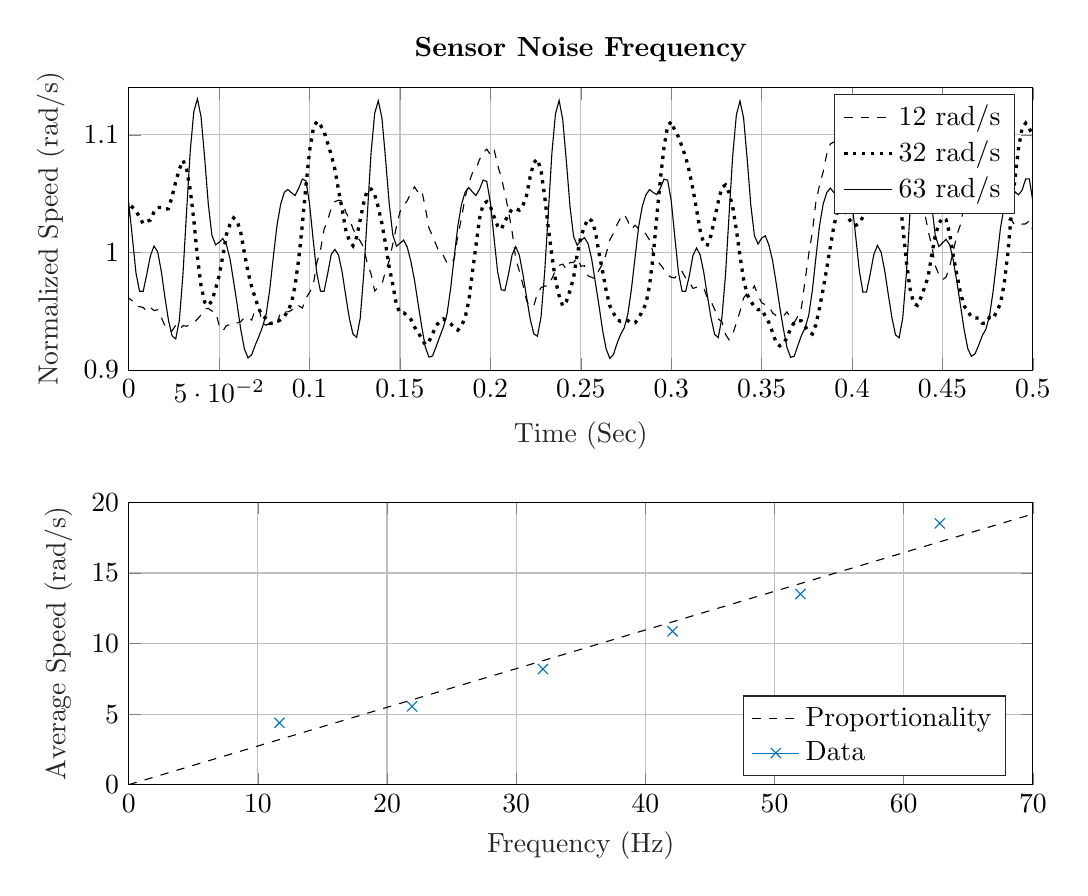
\begin{tikzpicture}

\begin{axis}[%
width=4.521in,
height=1.411in,
at={(0.758in,2.636in)},
scale only axis,
xmin=0,
xmax=0.5,
xlabel style={font=\color{white!15!black}},
xlabel={Time (Sec)},
ymin=0.9,
ymax=1.14,
ylabel style={font=\color{white!15!black}},
ylabel={Normalized Speed (rad/s)},
axis background/.style={fill=white},
title style={font=\bfseries},
title={Sensor Noise Frequency},
xmajorgrids,
ymajorgrids,
legend style={legend cell align=left, align=left, draw=white!15!black}
]
\addplot [color=black, dashed]
  table[row sep=crcr]{%
-0.913999915122986	1.04248678684235\\
-0.911999940872192	1.0288006067276\\
-0.909999907016754	1.01880359649658\\
-0.907999932765961	1.008171916008\\
-0.905999898910522	0.998658061027527\\
-0.903999924659729	0.994432389736176\\
-0.901999890804291	0.994536459445953\\
-0.899999916553497	0.991939187049866\\
-0.897999942302704	1.00002562999725\\
-0.895999908447266	1.00706624984741\\
-0.893999934196472	1.01876866817474\\
-0.891999900341034	1.03459167480469\\
-0.88999992609024	1.04635977745056\\
-0.887999892234802	1.06414306163788\\
-0.885999917984009	1.07502746582031\\
-0.883999943733215	1.07939410209656\\
-0.881999909877777	1.07989084720612\\
-0.879999935626984	1.08197724819183\\
-0.877999901771545	1.08335638046265\\
-0.875999927520752	1.08273303508759\\
-0.873999893665314	1.07941019535065\\
-0.87199991941452	1.07440507411957\\
-0.869999945163727	1.05291295051575\\
-0.867999911308289	1.03564774990082\\
-0.865999937057495	1.01683306694031\\
-0.863999903202057	0.998301446437836\\
-0.861999928951263	0.984731554985046\\
-0.859999895095825	0.969529449939728\\
-0.857999920845032	0.962417304515839\\
-0.855999946594238	0.961162626743317\\
-0.8539999127388	0.960611701011658\\
-0.851999938488007	0.95912766456604\\
-0.849999904632568	0.960530400276184\\
-0.847999930381775	0.964710295200348\\
-0.845999896526337	0.96358984708786\\
-0.843999922275543	0.971997618675232\\
-0.841999888420105	0.975650250911713\\
-0.839999914169312	0.987286448478699\\
-0.837999939918518	0.992793262004852\\
-0.83599990606308	0.991319835186005\\
-0.833999931812286	0.98442679643631\\
-0.831999897956848	0.983076691627502\\
-0.829999923706055	0.987927496433258\\
-0.827999949455261	0.990478992462158\\
-0.825999915599823	0.983912765979767\\
-0.82399994134903	0.976333737373352\\
-0.821999907493591	0.979126036167145\\
-0.819999933242798	0.976888000965118\\
-0.81799989938736	0.977390110492706\\
-0.815999925136566	0.988083958625793\\
-0.813999891281128	1.00214242935181\\
-0.811999917030334	1.01556670665741\\
-0.809999942779541	1.01849722862244\\
-0.807999908924103	1.0194296836853\\
-0.805999934673309	1.01556789875031\\
-0.803999900817871	1.01565527915955\\
-0.801999926567078	1.01514887809753\\
-0.799999952316284	1.01752197742462\\
-0.797999918460846	1.02797257900238\\
-0.795999944210052	1.02896392345428\\
-0.793999910354614	1.03254973888397\\
-0.791999936103821	1.02070152759552\\
-0.789999902248383	1.01171672344208\\
-0.787999927997589	0.997401773929596\\
-0.785999894142151	0.98454213142395\\
-0.783999919891357	0.980333805084229\\
-0.781999945640564	0.980849921703339\\
-0.779999911785126	0.982773959636688\\
-0.777999937534332	0.977645874023438\\
-0.775999903678894	0.987078487873077\\
-0.773999929428101	0.986196994781494\\
-0.771999955177307	0.98455798625946\\
-0.769999921321869	0.979641377925873\\
-0.767999947071075	0.974349021911621\\
-0.765999913215637	0.967883944511414\\
-0.763999938964844	0.968262493610382\\
-0.761999905109406	0.964055895805359\\
-0.759999930858612	0.964522242546082\\
-0.757999897003174	0.965184569358826\\
-0.75599992275238	0.960544764995575\\
-0.753999948501587	0.948430299758911\\
-0.751999914646149	0.944414258003235\\
-0.749999940395355	0.937276840209961\\
-0.747999906539917	0.934556305408478\\
-0.745999932289124	0.934016942977905\\
-0.74399995803833	0.933711290359497\\
-0.741999924182892	0.941099584102631\\
-0.739999890327454	0.948370933532715\\
-0.73799991607666	0.953267455101013\\
-0.735999941825867	0.961846470832825\\
-0.733999907970428	0.96600466966629\\
-0.731999933719635	0.970127522945404\\
-0.729999899864197	0.964107394218445\\
-0.727999925613403	0.958124279975891\\
-0.72599995136261	0.953354775905609\\
-0.723999917507172	0.956817150115967\\
-0.721999943256378	0.961602330207825\\
-0.71999990940094	0.951143860816956\\
-0.717999935150146	0.943107187747955\\
-0.715999960899353	0.943022608757019\\
-0.713999927043915	0.93791252374649\\
-0.711999893188477	0.938389241695404\\
-0.709999918937683	0.945781290531158\\
-0.70799994468689	0.947956323623657\\
-0.705999910831451	0.952935636043549\\
-0.703999936580658	0.971078932285309\\
-0.70199990272522	0.987119197845459\\
-0.699999928474426	1.00312292575836\\
-0.697999954223633	1.02896738052368\\
-0.695999920368195	1.04347014427185\\
-0.693999946117401	1.06065142154694\\
-0.691999912261963	1.07404577732086\\
-0.689999938011169	1.08230435848236\\
-0.687999963760376	1.08683514595032\\
-0.685999929904938	1.08881068229675\\
-0.6839998960495	1.09052491188049\\
-0.681999921798706	1.09764909744263\\
-0.679999947547913	1.09035980701447\\
-0.677999913692474	1.0859158039093\\
-0.675999939441681	1.07655334472656\\
-0.673999905586243	1.0667804479599\\
-0.671999931335449	1.05567395687103\\
-0.669999957084656	1.04664194583893\\
-0.667999923229218	1.04257929325104\\
-0.665999948978424	1.04373002052307\\
-0.663999915122986	1.05199944972992\\
-0.661999940872192	1.06152606010437\\
-0.659999966621399	1.07401561737061\\
-0.657999932765961	1.09097170829773\\
-0.655999898910522	1.10789883136749\\
-0.653999924659729	1.10050940513611\\
-0.651999950408936	1.0981776714325\\
-0.649999976158142	1.09608936309814\\
-0.647999942302704	1.09913313388824\\
-0.645999908447266	1.10236895084381\\
-0.643999934196472	1.08759331703186\\
-0.641999959945679	1.07299792766571\\
-0.63999992609024	1.05835998058319\\
-0.637999892234802	1.0470507144928\\
-0.635999917984009	1.02983129024506\\
-0.633999943733215	1.0186995267868\\
-0.631999969482422	1.00233280658722\\
-0.629999935626984	0.985852599143982\\
-0.627999901771545	0.977502524852753\\
-0.625999927520752	0.977802932262421\\
-0.623999953269959	0.980086505413055\\
-0.621999979019165	0.992142975330353\\
-0.619999945163727	1.00280630588531\\
-0.617999911308289	1.02122700214386\\
-0.615999937057495	1.03665697574615\\
-0.613999962806702	1.05284798145294\\
-0.611999928951263	1.0638986825943\\
-0.609999895095825	1.06311666965485\\
-0.607999920845032	1.06738448143005\\
-0.605999946594238	1.06943082809448\\
-0.603999972343445	1.07089745998383\\
-0.601999938488007	1.07635462284088\\
-0.599999904632568	1.06974065303802\\
-0.597999930381775	1.06565761566162\\
-0.595999956130981	1.06413495540619\\
-0.593999922275543	1.04951512813568\\
-0.59199994802475	1.03923845291138\\
-0.589999914169312	1.02825498580933\\
-0.587999939918518	1.01990914344788\\
-0.585999965667725	1.01757180690765\\
-0.583999931812286	1.01812100410461\\
-0.581999897956848	1.02136278152466\\
-0.579999923706055	1.02042865753174\\
-0.577999949455261	1.0177515745163\\
-0.575999975204468	1.02152621746063\\
-0.57399994134903	1.02547371387482\\
-0.571999907493591	1.02574944496155\\
-0.569999933242798	1.01731252670288\\
-0.567999958992004	1.01271212100983\\
-0.565999925136566	1.00695109367371\\
-0.563999950885773	0.999106347560883\\
-0.561999917030334	0.992854952812195\\
-0.559999942779541	0.990785598754883\\
-0.557999968528748	0.981589794158936\\
-0.555999934673309	0.980356752872467\\
-0.553999900817871	0.975615918636322\\
-0.551999926567078	0.969935178756714\\
-0.549999952316284	0.96676242351532\\
-0.547999978065491	0.957314252853394\\
-0.545999944210052	0.956986725330353\\
-0.543999910354614	0.962548911571503\\
-0.541999936103821	0.961157500743866\\
-0.539999961853027	0.962791621685028\\
-0.537999927997589	0.958740770816803\\
-0.535999953746796	0.959553122520447\\
-0.533999919891357	0.959251284599304\\
-0.531999945640564	0.955756902694702\\
-0.529999971389771	0.952280819416046\\
-0.527999937534332	0.947680473327637\\
-0.525999903678894	0.949821770191193\\
-0.523999929428101	0.948431193828583\\
-0.521999955177307	0.939483344554901\\
-0.519999980926514	0.943192720413208\\
-0.517999947071075	0.947168529033661\\
-0.515999913215637	0.939407765865326\\
-0.513999938964844	0.936623394489288\\
-0.51199996471405	0.933047890663147\\
-0.509999930858612	0.940127193927765\\
-0.507999956607819	0.940329611301422\\
-0.50599992275238	0.941026926040649\\
-0.503999948501587	0.940671801567078\\
-0.501999974250793	0.94459992647171\\
-0.499999940395355	0.941256821155548\\
-0.497999936342239	0.944868803024292\\
-0.495999932289124	0.937646448612213\\
-0.49399995803833	0.939038455486298\\
-0.491999953985214	0.950310230255127\\
-0.489999949932098	0.951791107654572\\
-0.487999945878983	0.951358437538147\\
-0.485999941825867	0.94450318813324\\
-0.483999937772751	0.941845595836639\\
-0.481999933719635	0.942461967468262\\
-0.479999959468842	0.94237208366394\\
-0.477999955415726	0.93851774930954\\
-0.47599995136261	0.932291805744171\\
-0.473999947309494	0.933448195457459\\
-0.471999943256378	0.935865163803101\\
-0.469999939203262	0.938035845756531\\
-0.467999935150146	0.941715955734253\\
-0.465999960899353	0.947462975978851\\
-0.463999956846237	0.956096053123474\\
-0.461999952793121	0.952599406242371\\
-0.459999948740005	0.946683824062347\\
-0.45799994468689	0.941836595535278\\
-0.455999940633774	0.938347101211548\\
-0.453999936580658	0.945106983184814\\
-0.451999932527542	0.947009205818176\\
-0.449999958276749	0.945289790630341\\
-0.447999954223633	0.955624580383301\\
-0.445999950170517	0.959007084369659\\
-0.443999946117401	0.957664132118225\\
-0.441999942064285	0.956454336643219\\
-0.439999938011169	0.957694888114929\\
-0.437999933958054	0.957375824451447\\
-0.43599995970726	0.971438884735107\\
-0.433999955654144	0.990105032920837\\
-0.431999951601028	1.00773072242737\\
-0.429999947547913	1.01880371570587\\
-0.427999943494797	1.02653658390045\\
-0.425999939441681	1.03032803535461\\
-0.423999935388565	1.0371196269989\\
-0.421999961137772	1.04231750965118\\
-0.419999957084656	1.04163229465485\\
-0.41799995303154	1.04497420787811\\
-0.415999948978424	1.03680872917175\\
-0.413999944925308	1.02730309963226\\
-0.411999940872192	1.01381182670593\\
-0.409999966621399	0.99922651052475\\
-0.407999932765961	0.991999745368958\\
-0.405999958515167	0.986766397953033\\
-0.403999924659729	0.986094892024994\\
-0.401999950408936	0.982529699802399\\
-0.399999976158142	0.978116452693939\\
-0.397999942302704	0.977194249629974\\
-0.39599996805191	0.983322978019714\\
-0.393999934196472	0.994232058525085\\
-0.391999959945679	1.00443387031555\\
-0.38999992609024	1.01948845386505\\
-0.387999951839447	1.02802455425262\\
-0.385999977588654	1.04180002212524\\
-0.383999943733215	1.04713046550751\\
-0.381999969482422	1.0566098690033\\
-0.379999935626984	1.05775952339172\\
-0.37799996137619	1.05074870586395\\
-0.375999927520752	1.04613828659058\\
-0.373999953269959	1.03345227241516\\
-0.371999979019165	1.02693843841553\\
-0.369999945163727	1.01854467391968\\
-0.367999970912933	1.0032662153244\\
-0.365999937057495	0.994151294231415\\
-0.363999962806702	0.984681963920593\\
-0.361999928951263	0.98495751619339\\
-0.35999995470047	0.991129159927368\\
-0.357999980449677	1.00169336795807\\
-0.355999946594238	1.01679539680481\\
-0.353999972343445	1.03230929374695\\
-0.351999938488007	1.04729080200195\\
-0.349999964237213	1.06375408172607\\
-0.347999930381775	1.07159447669983\\
-0.345999956130981	1.07687342166901\\
-0.343999981880188	1.08168196678162\\
-0.34199994802475	1.08496999740601\\
-0.339999973773956	1.08541929721832\\
-0.337999939918518	1.08679842948914\\
-0.335999965667725	1.07889008522034\\
-0.333999931812286	1.06984150409698\\
-0.331999957561493	1.06461262702942\\
-0.329999983310699	1.04956603050232\\
-0.327999949455261	1.03488445281982\\
-0.325999975204468	1.01447820663452\\
-0.32399994134903	0.996839940547943\\
-0.321999967098236	0.980730056762695\\
-0.319999933242798	0.970184564590454\\
-0.317999958992004	0.957496166229248\\
-0.315999984741211	0.952145576477051\\
-0.313999950885773	0.953785479068756\\
-0.311999976634979	0.962118208408356\\
-0.309999942779541	0.965768039226532\\
-0.307999968528748	0.972938418388367\\
-0.305999934673309	0.975200712680817\\
-0.303999960422516	0.983118712902069\\
-0.301999986171722	0.989799797534943\\
-0.299999952316284	0.989727139472961\\
-0.297999978065491	0.994354605674744\\
-0.295999944210052	0.994868576526642\\
-0.293999969959259	0.993888020515442\\
-0.291999936103821	0.986606419086456\\
-0.289999961853027	0.985396862030029\\
-0.287999987602234	0.979420781135559\\
-0.285999953746796	0.981405675411224\\
-0.283999979496002	0.988134205341339\\
-0.281999945640564	0.987276554107666\\
-0.279999971389771	0.989872992038727\\
-0.277999937534332	0.99271297454834\\
-0.275999963283539	0.992976486682892\\
-0.273999929428101	1.00046706199646\\
-0.271999955177307	1.00516223907471\\
-0.269999980926514	1.0104067325592\\
-0.267999947071075	1.02323591709137\\
-0.265999972820282	1.02508640289307\\
-0.263999938964844	1.0280739068985\\
-0.26199996471405	1.02853894233704\\
-0.259999930858612	1.03042960166931\\
-0.257999956607819	1.02828347682953\\
-0.255999982357025	1.02959287166595\\
-0.253999948501587	1.01922917366028\\
-0.251999974250793	1.00918841362\\
-0.249999940395355	1.00499403476715\\
-0.247999966144562	0.999039590358734\\
-0.245999932289124	0.989155471324921\\
-0.24399995803833	0.982941031455994\\
-0.241999983787537	0.978604972362518\\
-0.239999949932098	0.976638078689575\\
-0.237999975681305	0.978825151920319\\
-0.235999941825867	0.982147812843323\\
-0.233999967575073	0.987392783164978\\
-0.231999933719635	0.988442182540894\\
-0.229999959468842	0.97978001832962\\
-0.227999985218048	0.974391758441925\\
-0.22599995136261	0.973639786243439\\
-0.223999977111816	0.968376815319061\\
-0.221999943256378	0.963754057884216\\
-0.219999969005585	0.959616303443909\\
-0.217999935150146	0.964053869247437\\
-0.215999960899353	0.955075204372406\\
-0.21399998664856	0.951394259929657\\
-0.211999952793121	0.944410085678101\\
-0.209999978542328	0.934351325035095\\
-0.20799994468689	0.929500758647919\\
-0.205999970436096	0.931942284107208\\
-0.203999936580658	0.934246838092804\\
-0.201999962329865	0.944857478141785\\
-0.199999988079071	0.951729416847229\\
-0.197999954223633	0.968312799930573\\
-0.195999979972839	0.970074117183685\\
-0.193999946117401	0.967599630355835\\
-0.191999971866608	0.969040036201477\\
-0.189999938011169	0.961207985877991\\
-0.187999963760376	0.955723226070404\\
-0.185999989509583	0.954508602619171\\
-0.183999955654144	0.953518688678741\\
-0.181999981403351	0.948645055294037\\
-0.179999947547913	0.947712302207947\\
-0.177999973297119	0.945281207561493\\
-0.175999939441681	0.94256454706192\\
-0.173999965190887	0.944684326648712\\
-0.171999990940094	0.945982933044434\\
-0.169999957084656	0.947454690933228\\
-0.167999982833862	0.959629952907562\\
-0.165999948978424	0.968074977397919\\
-0.163999974727631	0.982997298240662\\
-0.161999940872192	0.999963045120239\\
-0.159999966621399	1.01664805412292\\
-0.157999992370605	1.03986752033234\\
-0.155999958515167	1.05850207805634\\
-0.153999984264374	1.07335042953491\\
-0.151999950408936	1.08999788761139\\
-0.149999976158142	1.09613800048828\\
-0.147999942302704	1.09273302555084\\
-0.14599996805191	1.09054553508759\\
-0.143999993801117	1.09255683422089\\
-0.141999959945679	1.09195733070374\\
-0.139999985694885	1.08990597724915\\
-0.137999951839447	1.0806736946106\\
-0.135999977588654	1.06652617454529\\
-0.133999943733215	1.05658423900604\\
-0.131999969482422	1.04311728477478\\
-0.129999995231628	1.05190110206604\\
-0.12799996137619	1.04940605163574\\
-0.125999987125397	1.0533492565155\\
-0.123999953269959	1.0621178150177\\
-0.121999979019165	1.06889986991882\\
-0.119999945163727	1.08074486255646\\
-0.117999970912933	1.09320473670959\\
-0.11599999666214	1.09600436687469\\
-0.113999962806702	1.10357046127319\\
-0.111999988555908	1.10387456417084\\
-0.10999995470047	1.1036456823349\\
-0.107999980449677	1.10342812538147\\
-0.105999946594238	1.09411752223969\\
-0.103999972343445	1.08526623249054\\
-0.101999998092651	1.06560051441193\\
-0.0999999642372131	1.04895901679993\\
-0.0979999899864197	1.03132200241089\\
-0.0959999561309814	1.01589953899384\\
-0.093999981880188	1.00050485134125\\
-0.0919999480247498	0.986001253128052\\
-0.0899999737739563	0.977716147899628\\
-0.0879999995231628	0.976053655147552\\
-0.0859999656677246	0.987423479557037\\
-0.0839999914169312	0.999946236610413\\
-0.0819999575614929	1.00913298130035\\
-0.0799999833106995	1.01098418235779\\
-0.0779999494552612	1.02005815505981\\
-0.0759999752044678	1.04047882556915\\
-0.0740000009536743	1.0494419336319\\
-0.0719999670982361	1.06322550773621\\
-0.0699999928474426	1.07231116294861\\
-0.0679999589920044	1.07896888256073\\
-0.0659999847412109	1.08039116859436\\
-0.0639999508857727	1.07897591590881\\
-0.0619999766349792	1.07549941539764\\
-0.0600000023841858	1.06631016731262\\
-0.0579999685287476	1.05474388599396\\
-0.0559999942779541	1.04748237133026\\
-0.0539999604225159	1.03725528717041\\
-0.0519999861717224	1.03142249584198\\
-0.0499999523162842	1.02488946914673\\
-0.0479999780654907	1.02138292789459\\
-0.0460000038146973	1.02501726150513\\
-0.043999969959259	1.02236592769623\\
-0.0419999957084656	1.02416300773621\\
-0.0399999618530273	1.02127146720886\\
-0.0379999876022339	1.01822555065155\\
-0.0359999537467957	1.01851046085358\\
-0.0339999794960022	1.0192756652832\\
-0.0320000052452087	1.01374566555023\\
-0.0299999713897705	1.01145672798157\\
-0.0279999971389771	1.00886487960815\\
-0.0259999632835388	1.00177836418152\\
-0.0239999890327454	1.00438392162323\\
-0.0219999551773071	1.002774477005\\
-0.0199999809265137	0.992451250553131\\
-0.0180000066757202	0.984892666339874\\
-0.015999972820282	0.975156724452972\\
-0.0139999985694885	0.970122992992401\\
-0.0119999647140503	0.964229285717011\\
-0.00999999046325684	0.957111001014709\\
-0.0079999566078186	0.951591789722443\\
-0.00599998235702515	0.955753803253174\\
-0.00399994850158691	0.951063811779022\\
-0.00199997425079346	0.960309863090515\\
0	0.961234271526337\\
0.00200003385543823	0.958853542804718\\
0.00400000810623169	0.954118371009827\\
0.00600004196166992	0.953964233398438\\
0.00800001621246338	0.953266561031342\\
0.0100000500679016	0.950039505958557\\
0.0120000243186951	0.953184366226196\\
0.0139999985694885	0.950558185577393\\
0.0160000324249268	0.951361000537872\\
0.0180000066757202	0.944791197776794\\
0.0200000405311584	0.937698900699615\\
0.0220000147819519	0.933310747146606\\
0.0240000486373901	0.933488547801971\\
0.0260000228881836	0.9380122423172\\
0.0279999971389771	0.934478878974915\\
0.0300000309944153	0.937808692455292\\
0.0320000052452087	0.937274396419525\\
0.034000039100647	0.938925683498383\\
0.0360000133514404	0.940070271492004\\
0.0380000472068787	0.943447172641754\\
0.0400000214576721	0.946890473365784\\
0.0419999957084656	0.952084362506866\\
0.0440000295639038	0.952405154705048\\
0.0460000038146973	0.950207114219666\\
0.0480000376701355	0.949744284152985\\
0.050000011920929	0.937927424907684\\
0.0520000457763672	0.933067083358765\\
0.0540000200271606	0.937793672084808\\
0.0559999942779541	0.938704550266266\\
0.0580000281333923	0.940874695777893\\
0.0600000023841858	0.940113008022308\\
0.062000036239624	0.941258788108826\\
0.0640000104904175	0.944754540920258\\
0.0660000443458557	0.944860577583313\\
0.0680000185966492	0.942520558834076\\
0.0699999928474426	0.951976776123047\\
0.0720000267028809	0.952059864997864\\
0.0740000009536743	0.939625084400177\\
0.0760000348091125	0.938099086284637\\
0.078000009059906	0.94008880853653\\
0.0800000429153442	0.940523684024811\\
0.0820000171661377	0.938807606697083\\
0.0839999914169312	0.950027406215668\\
0.0860000252723694	0.94952267408371\\
0.0880000591278076	0.949490666389465\\
0.0900000333786011	0.950709342956543\\
0.0920000076293945	0.955597937107086\\
0.093999981880188	0.954667806625366\\
0.0959999561309814	0.952723503112793\\
0.0980000495910645	0.961145102977753\\
0.100000023841858	0.966026842594147\\
0.101999998092651	0.972124218940735\\
0.103999972343445	0.991118967533112\\
0.106000065803528	1.00186824798584\\
0.108000040054321	1.01963007450104\\
0.110000014305115	1.02723860740662\\
0.111999988555908	1.03806209564209\\
0.113999962806702	1.04325830936432\\
0.116000056266785	1.04451084136963\\
0.118000030517578	1.04380476474762\\
0.120000004768372	1.03423738479614\\
0.121999979019165	1.02877116203308\\
0.124000072479248	1.02026188373566\\
0.126000046730042	1.0144237279892\\
0.128000020980835	1.00966334342957\\
0.129999995231628	1.00402104854584\\
0.131999969482422	0.990151107311249\\
0.134000062942505	0.981755673885345\\
0.136000037193298	0.967369198799133\\
0.138000011444092	0.970191955566406\\
0.139999985694885	0.972881019115448\\
0.141999959945679	0.984279155731201\\
0.144000053405762	0.992880046367645\\
0.146000027656555	1.00706744194031\\
0.148000001907349	1.02178978919983\\
0.149999976158142	1.03465461730957\\
0.152000069618225	1.0402272939682\\
0.154000043869019	1.04395818710327\\
0.156000018119812	1.05054032802582\\
0.157999992370605	1.05574285984039\\
0.159999966621399	1.05121397972107\\
0.162000060081482	1.05315577983856\\
0.164000034332275	1.0381373167038\\
0.166000008583069	1.02091574668884\\
0.167999982833862	1.01394867897034\\
0.169999957084656	1.00645482540131\\
0.172000050544739	0.998884081840515\\
0.174000024795532	0.997359156608582\\
0.175999999046326	0.991209268569946\\
0.177999973297119	0.989955127239227\\
0.180000066757202	0.994805872440338\\
0.182000041007996	1.01447892189026\\
0.184000015258789	1.02909719944\\
0.185999989509583	1.04681015014648\\
0.187999963760376	1.05856502056122\\
0.190000057220459	1.06754660606384\\
0.192000031471252	1.07089841365814\\
0.194000005722046	1.07915902137756\\
0.195999979972839	1.08522212505341\\
0.197999954223633	1.08786797523499\\
0.200000047683716	1.08318746089935\\
0.202000021934509	1.0878814458847\\
0.203999996185303	1.07429707050323\\
0.205999970436096	1.06393432617188\\
0.208000063896179	1.05054497718811\\
0.210000038146973	1.03521645069122\\
0.212000012397766	1.01789367198944\\
0.21399998664856	0.99480128288269\\
0.215999960899353	0.98408180475235\\
0.218000054359436	0.972497522830963\\
0.220000028610229	0.959079146385193\\
0.222000002861023	0.953758120536804\\
0.223999977111816	0.954571187496185\\
0.22599995136261	0.965435981750488\\
0.228000044822693	0.970079302787781\\
0.230000019073486	0.971489667892456\\
0.23199999332428	0.971561431884766\\
0.233999967575073	0.977900207042694\\
0.236000061035156	0.984672904014587\\
0.23800003528595	0.98910790681839\\
0.240000009536743	0.990069091320038\\
0.241999983787537	0.985760271549225\\
0.24399995803833	0.991446793079376\\
0.246000051498413	0.991460382938385\\
0.248000025749207	0.995577037334442\\
0.25	0.988312423229218\\
0.251999974250793	0.988698244094849\\
0.253999948501587	0.980013906955719\\
0.25600004196167	0.978891253471375\\
0.258000016212463	0.977605521678925\\
0.259999990463257	0.984797179698944\\
0.26199996471405	0.990227162837982\\
0.264000058174133	0.998951733112335\\
0.266000032424927	1.01060795783997\\
0.26800000667572	1.01624882221222\\
0.269999980926514	1.02366554737091\\
0.271999955177307	1.02964079380035\\
0.27400004863739	1.03267621994019\\
0.276000022888184	1.02673053741455\\
0.277999997138977	1.01985597610474\\
0.279999971389771	1.02320396900177\\
0.281999945640564	1.01998746395111\\
0.284000039100647	1.01960718631744\\
0.28600001335144	1.01552546024323\\
0.287999987602234	1.01062917709351\\
0.289999961853027	0.999788999557495\\
0.29200005531311	0.993268072605133\\
0.294000029563904	0.989749372005463\\
0.296000003814697	0.985570251941681\\
0.297999978065491	0.980940163135529\\
0.299999952316284	0.978882610797882\\
0.302000045776367	0.978420555591583\\
0.304000020027161	0.983744978904724\\
0.305999994277954	0.983897805213928\\
0.307999968528748	0.978059411048889\\
0.309999942779541	0.975051581859589\\
0.312000036239624	0.969505131244659\\
0.314000010490417	0.970455050468445\\
0.315999984741211	0.970049202442169\\
0.317999958992004	0.969896674156189\\
0.320000052452087	0.961117684841156\\
0.322000026702881	0.958277702331543\\
0.324000000953674	0.951639711856842\\
0.325999975204468	0.943511843681335\\
0.327999949455261	0.941128671169281\\
0.330000042915344	0.930427432060242\\
0.332000017166138	0.925670325756073\\
0.333999991416931	0.930353760719299\\
0.335999965667725	0.94013637304306\\
0.337999939918518	0.949815928936005\\
0.340000033378601	0.961268365383148\\
0.342000007629395	0.96542763710022\\
0.343999981880188	0.966427028179169\\
0.345999956130981	0.971584379673004\\
0.348000049591064	0.96346914768219\\
0.350000023841858	0.95733118057251\\
0.351999998092651	0.955462217330933\\
0.353999972343445	0.954398155212402\\
0.355999946594238	0.948629260063171\\
0.358000040054321	0.946322202682495\\
0.360000014305115	0.94571053981781\\
0.361999988555908	0.945834219455719\\
0.363999962806702	0.949534475803375\\
0.366000056266785	0.944045186042786\\
0.368000030517578	0.940338611602783\\
0.370000004768372	0.945727407932281\\
0.371999979019165	0.953244388103485\\
0.373999953269959	0.976202607154846\\
0.376000046730042	0.998181283473969\\
0.378000020980835	1.01715290546417\\
0.379999995231628	1.04324531555176\\
0.381999969482422	1.05721306800842\\
0.383999943733215	1.06864082813263\\
0.386000037193298	1.08381187915802\\
0.388000011444092	1.0923730134964\\
0.389999985694885	1.09403002262115\\
0.391999959945679	1.09275102615356\\
0.394000053405762	1.09804356098175\\
0.396000027656555	1.09270298480988\\
0.398000001907349	1.08469271659851\\
0.399999976158142	1.07470595836639\\
0.401999950408936	1.06503713130951\\
0.404000043869019	1.05822741985321\\
0.406000018119812	1.04884111881256\\
0.407999992370605	1.04602158069611\\
0.409999966621399	1.04702508449554\\
0.411999940872192	1.04565227031708\\
0.414000034332275	1.05394446849823\\
0.416000008583069	1.06712448596954\\
0.417999982833862	1.07901120185852\\
0.419999957084656	1.08921253681183\\
0.422000050544739	1.09755527973175\\
0.424000024795532	1.10142958164215\\
0.425999999046326	1.09873175621033\\
0.427999973297119	1.10396182537079\\
0.429999947547913	1.10364258289337\\
0.432000041007996	1.09958481788635\\
0.434000015258789	1.08605694770813\\
0.435999989509583	1.07218134403229\\
0.437999963760376	1.05064797401428\\
0.439999938011169	1.03506541252136\\
0.442000031471252	1.01861846446991\\
0.444000005722046	1.00622510910034\\
0.445999979972839	0.988791406154633\\
0.447999954223633	0.981088221073151\\
0.450000047683716	0.976828336715698\\
0.452000021934509	0.979184210300446\\
0.453999996185303	0.988022804260254\\
0.455999970436096	1.00162327289581\\
0.45799994468689	1.01511108875275\\
0.460000038146973	1.0242018699646\\
0.462000012397766	1.04074335098267\\
0.46399998664856	1.04943144321442\\
0.465999960899353	1.06092607975006\\
0.467999935150146	1.06712603569031\\
0.470000028610229	1.07225716114044\\
0.472000002861023	1.06783854961395\\
0.473999977111816	1.06934010982513\\
0.47599995136261	1.07618713378906\\
0.478000044822693	1.07351326942444\\
0.480000019073486	1.0629985332489\\
0.48199999332428	1.05122649669647\\
0.483999967575073	1.03842532634735\\
0.485999941825867	1.02773058414459\\
0.48800003528595	1.028235912323\\
0.490000009536743	1.02300941944122\\
0.491999983787537	1.02397906780243\\
0.49399995803833	1.02414298057556\\
0.495999932289124	1.02428030967712\\
0.498000025749207	1.02700579166412\\
0.5	1.0187087059021\\
0.501999974250793	1.02043783664703\\
0.503999948501587	1.01855134963989\\
0.50600004196167	1.01506555080414\\
0.508000016212463	1.01350665092468\\
0.509999990463257	1.00714695453644\\
0.51199996471405	1.00225031375885\\
0.513999938964844	1.00029611587524\\
0.516000032424927	1.00143349170685\\
0.51800000667572	0.993030488491058\\
0.519999980926514	0.988499045372009\\
0.521999955177307	0.979645133018494\\
0.523999929428101	0.9685018658638\\
0.526000022888184	0.966599762439728\\
0.527999997138977	0.956921100616455\\
0.529999971389771	0.950867891311646\\
0.531999945640564	0.955868244171143\\
0.534000039100647	0.957076609134674\\
0.53600001335144	0.962902903556824\\
0.537999987602234	0.962953150272369\\
0.539999961853027	0.961465954780579\\
0.541999936103821	0.962167918682098\\
0.544000029563904	0.96065217256546\\
0.546000003814697	0.959832787513733\\
0.547999978065491	0.95546567440033\\
0.549999952316284	0.945148348808289\\
0.551999926567078	0.943750321865082\\
0.554000020027161	0.935999631881714\\
0.555999994277954	0.933246493339539\\
0.557999968528748	0.934177339076996\\
0.559999942779541	0.939428091049194\\
0.562000036239624	0.935884177684784\\
0.564000010490417	0.935683012008667\\
0.565999984741211	0.939979553222656\\
0.567999958992004	0.938901305198669\\
0.569999933242798	0.940924227237701\\
0.572000026702881	0.944099962711334\\
0.574000000953674	0.948057532310486\\
0.575999975204468	0.950276613235474\\
0.577999949455261	0.945069432258606\\
0.579999923706055	0.944823384284973\\
0.582000017166138	0.9445521235466\\
0.583999991416931	0.941589891910553\\
0.585999965667725	0.941863536834717\\
0.587999939918518	0.940361082553864\\
0.590000033378601	0.943114578723907\\
0.592000007629395	0.946915626525879\\
0.593999981880188	0.941349923610687\\
0.595999956130981	0.94331568479538\\
0.597999930381775	0.93927276134491\\
0.600000023841858	0.933513522148132\\
0.601999998092651	0.931988000869751\\
0.603999972343445	0.933093249797821\\
0.605999946594238	0.941901922225952\\
0.607999920845032	0.949162662029266\\
0.610000014305115	0.949025213718414\\
0.611999988555908	0.951863348484039\\
0.613999962806702	0.947402477264404\\
0.615999937057495	0.944091439247131\\
0.618000030517578	0.944007337093353\\
0.620000004768372	0.942773222923279\\
0.621999979019165	0.939519643783569\\
0.623999953269959	0.945496082305908\\
0.625999927520752	0.95040637254715\\
0.628000020980835	0.949775993824005\\
0.629999995231628	0.948399722576141\\
0.631999969482422	0.948607265949249\\
0.633999943733215	0.955478072166443\\
0.636000037193298	0.961384296417236\\
0.638000011444092	0.963466227054596\\
0.639999985694885	0.966148495674133\\
0.641999959945679	0.98374330997467\\
0.643999934196472	0.997786581516266\\
0.646000027656555	1.01392841339111\\
0.648000001907349	1.02648591995239\\
0.649999976158142	1.03785800933838\\
0.651999950408936	1.03928339481354\\
0.653999924659729	1.04485082626343\\
0.656000018119812	1.03851091861725\\
0.657999992370605	1.03595948219299\\
0.659999966621399	1.02732694149017\\
0.661999940872192	1.02001941204071\\
0.664000034332275	1.01304578781128\\
0.666000008583069	1.00986111164093\\
0.667999982833862	1.00033831596375\\
0.669999957084656	0.990762889385223\\
0.671999931335449	0.988004446029663\\
0.674000024795532	0.984189689159393\\
0.675999999046326	0.979822039604187\\
0.677999973297119	0.97394859790802\\
0.679999947547913	0.976758182048798\\
0.681999921798706	0.991407096385956\\
0.684000015258789	0.999426305294037\\
0.685999989509583	1.01705932617188\\
0.687999963760376	1.03204619884491\\
0.689999938011169	1.03687357902527\\
0.692000031471252	1.04348111152649\\
0.694000005722046	1.04605507850647\\
0.695999979972839	1.04583072662354\\
0.697999954223633	1.04863727092743\\
0.699999928474426	1.04588770866394\\
0.702000021934509	1.039705991745\\
0.703999996185303	1.0296790599823\\
0.705999970436096	1.01498126983643\\
0.70799994468689	1.00895297527313\\
0.709999918937683	1.00348174571991\\
0.712000012397766	0.998184263706207\\
0.71399998664856	0.987310826778412\\
0.715999960899353	0.987154185771942\\
0.717999935150146	0.993132054805756\\
0.720000028610229	1.00451266765594\\
0.722000002861023	1.01661038398743\\
0.723999977111816	1.03265583515167\\
0.72599995136261	1.0469012260437\\
0.727999925613403	1.07182443141937\\
0.730000019073486	1.08734273910522\\
0.73199999332428	1.08530580997467\\
0.733999967575073	1.09126961231232\\
0.735999941825867	1.07987546920776\\
0.73799991607666	1.07959806919098\\
0.740000009536743	1.07882285118103\\
0.741999983787537	1.06813538074493\\
0.74399995803833	1.06016182899475\\
0.745999932289124	1.05286419391632\\
0.748000025749207	1.03989660739899\\
0.75	1.02238285541534\\
0.751999974250793	1.01090812683105\\
0.753999948501587	0.996336817741394\\
0.75599992275238	0.9760901927948\\
0.758000016212463	0.965983092784882\\
0.759999990463257	0.952800035476685\\
0.76199996471405	0.947998285293579\\
0.763999938964844	0.951418459415436\\
0.765999913215637	0.963438749313354\\
0.76800000667572	0.973842024803162\\
0.769999980926514	0.979886889457703\\
0.771999955177307	0.977900564670563\\
0.773999929428101	0.979844272136688\\
0.776000022888184	0.986758768558502\\
0.777999997138977	0.987173318862915\\
0.779999971389771	0.990115880966187\\
0.781999945640564	0.987450957298279\\
0.783999919891357	0.988980948925018\\
0.78600001335144	0.985507071018219\\
0.787999987602234	0.988302052021027\\
0.789999961853027	0.987037241458893\\
0.791999936103821	0.984885811805725\\
0.793999910354614	0.982787013053894\\
0.796000003814697	0.982726871967316\\
0.797999978065491	0.989699840545654\\
0.799999952316284	0.990067720413208\\
0.801999926567078	0.996708750724792\\
0.804000020027161	1.00528419017792\\
0.805999994277954	1.01129233837128\\
0.807999968528748	1.02260792255402\\
0.809999942779541	1.02549362182617\\
0.811999917030334	1.0241471529007\\
0.814000010490417	1.02748906612396\\
0.815999984741211	1.02565610408783\\
0.817999958992004	1.02548682689667\\
0.819999933242798	1.02648818492889\\
0.821999907493591	1.02041661739349\\
0.824000000953674	1.0179351568222\\
0.825999975204468	1.01468443870544\\
0.827999949455261	1.0013724565506\\
0.829999923706055	1.00260412693024\\
0.832000017166138	0.989564299583435\\
0.833999991416931	0.973388612270355\\
0.835999965667725	0.964816510677338\\
0.837999939918518	0.968971252441406\\
0.839999914169312	0.978343486785889\\
0.842000007629395	0.983419001102448\\
0.843999981880188	0.99162769317627\\
0.845999956130981	0.990941524505615\\
0.847999930381775	0.989210784435272\\
0.849999904632568	0.98698890209198\\
0.851999998092651	0.976547300815582\\
0.853999972343445	0.96695351600647\\
0.855999946594238	0.954539179801941\\
0.857999920845032	0.95061457157135\\
0.860000014305115	0.952939450740814\\
0.861999988555908	0.948725759983063\\
0.863999962806702	0.948522865772247\\
0.865999937057495	0.941645801067352\\
0.867999911308289	0.937188446521759\\
0.870000004768372	0.93752384185791\\
0.871999979019165	0.93528801202774\\
0.873999953269959	0.935295641422272\\
0.875999927520752	0.943521201610565\\
0.877999901771545	0.953722238540649\\
0.879999995231628	0.959553599357605\\
0.881999969482422	0.964584052562714\\
0.883999943733215	0.967517197132111\\
0.885999917984009	0.967613637447357\\
0.888000011444092	0.960205435752869\\
0.889999985694885	0.957096517086029\\
0.891999959945679	0.956766724586487\\
0.893999934196472	0.950862169265747\\
0.895999908447266	0.94447523355484\\
0.898000001907349	0.940321743488312\\
0.899999976158142	0.944951415061951\\
0.901999950408936	0.95098739862442\\
0.903999924659729	0.949872970581055\\
0.906000018119812	0.94869065284729\\
0.907999992370605	0.948616206645966\\
0.909999966621399	0.956115126609802\\
0.911999940872192	0.963418424129486\\
0.913999915122986	0.982791423797607\\
0.916000008583069	1.00051856040955\\
0.917999982833862	1.02568817138672\\
0.919999957084656	1.05381977558136\\
0.921999931335449	1.0706832408905\\
0.923999905586243	1.08064496517181\\
0.925999999046326	1.09425783157349\\
0.927999973297119	1.09673321247101\\
0.929999947547913	1.09301793575287\\
0.931999921798706	1.09725880622864\\
0.934000015258789	1.08857715129852\\
0.935999989509583	1.09095728397369\\
0.937999963760376	1.08122634887695\\
0.939999938011169	1.06866633892059\\
0.941999912261963	1.06769800186157\\
0.944000005722046	1.05406212806702\\
0.945999979972839	1.0510082244873\\
0.947999954223633	1.04782700538635\\
0.949999928474426	1.04719090461731\\
0.95199990272522	1.05088925361633\\
0.953999996185303	1.0614058971405\\
0.955999970436096	1.07084369659424\\
0.95799994468689	1.08936333656311\\
0.959999918937683	1.10163426399231\\
0.962000012397766	1.10672581195831\\
0.96399998664856	1.10437405109406\\
0.965999960899353	1.09571194648743\\
0.967999935150146	1.09564852714539\\
0.96999990940094	1.09700751304626\\
0.972000002861023	1.0864360332489\\
0.973999977111816	1.07855272293091\\
0.97599995136261	1.06604361534119\\
0.977999925613403	1.04625606536865\\
0.979999899864197	1.02511119842529\\
0.98199999332428	1.01008522510529\\
0.983999967575073	0.991281509399414\\
0.985999941825867	0.97905033826828\\
0.98799991607666	0.98417592048645\\
0.990000009536743	0.981370985507965\\
0.991999983787537	0.987090349197388\\
0.99399995803833	0.998043358325958\\
0.995999932289124	1.00951218605042\\
0.997999906539917	1.02450680732727\\
1	1.03720903396606\\
1.00199997425079	1.04846739768982\\
1.00399994850159	1.05870306491852\\
1.00599992275238	1.06184709072113\\
1.00799989700317	1.06832826137543\\
1.00999999046326	1.07124650478363\\
1.01199996471405	1.07718801498413\\
1.01399993896484	1.07433903217316\\
1.01599991321564	1.06531250476837\\
1.01800000667572	1.06144082546234\\
1.01999998092651	1.05432498455048\\
1.02199995517731	1.04713010787964\\
1.0239999294281	1.04328942298889\\
1.02599990367889	1.03219759464264\\
1.02799999713898	1.03060352802277\\
1.02999997138977	1.01827657222748\\
1.03199994564056	1.02229356765747\\
1.03399991989136	1.01928102970123\\
1.03599989414215	1.02230143547058\\
1.03799998760223	1.02204215526581\\
1.03999996185303	1.02179741859436\\
1.04199993610382	1.02442908287048\\
1.04399991035461	1.02061927318573\\
1.0460000038147	1.02193033695221\\
1.04799997806549	1.01757323741913\\
1.04999995231628	1.00671744346619\\
1.05199992656708	1.00014126300812\\
1.05399990081787	0.997239112854004\\
1.05599999427795	0.994046688079834\\
1.05799996852875	0.989280998706818\\
1.05999994277954	0.979978859424591\\
1.06199991703033	0.97452700138092\\
1.06399989128113	0.965708613395691\\
1.06599998474121	0.963255167007446\\
1.067999958992	0.956060171127319\\
1.0699999332428	0.957307875156403\\
1.07199990749359	0.95701801776886\\
1.07400000095367	0.957207322120667\\
1.07599997520447	0.95695698261261\\
1.07799994945526	0.956115245819092\\
1.07999992370605	0.96211302280426\\
1.08199989795685	0.963892817497253\\
1.08399999141693	0.961753785610199\\
1.08599996566772	0.95685613155365\\
1.08799993991852	0.954437792301178\\
1.0900000333786	0.951437890529633\\
1.09199988842011	0.948987305164337\\
1.09399998188019	0.935255169868469\\
1.09599983692169	0.93159556388855\\
1.09799993038177	0.936565756797791\\
1.10000002384186	0.937406122684479\\
1.10199987888336	0.937357723712921\\
1.10399997234344	0.942746102809906\\
1.10599982738495	0.943609595298767\\
1.10799992084503	0.937426924705505\\
1.11000001430511	0.937573730945587\\
1.11199986934662	0.944932818412781\\
1.1139999628067	0.949122488498688\\
1.11600005626678	0.943567276000977\\
1.11799991130829	0.945636570453644\\
1.12000000476837	0.94495415687561\\
1.12199985980988	0.940714538097382\\
1.12399995326996	0.949318766593933\\
1.12600004673004	0.950204610824585\\
1.12799990177155	0.947174847126007\\
1.12999999523163	0.940040946006775\\
1.13199985027313	0.940234899520874\\
};
\addlegendentry{12 rad/s}

\addplot [color=black, dotted, line width=1.2pt]
  table[row sep=crcr]{%
-0.639999985694885	0.990998268127441\\
-0.638000011444092	0.97657310962677\\
-0.635999977588654	0.962053537368774\\
-0.63400000333786	0.954626858234406\\
-0.631999969482422	0.949259221553802\\
-0.629999995231628	0.948485553264618\\
-0.62799996137619	0.948229312896729\\
-0.625999987125397	0.945712208747864\\
-0.624000012874603	0.936781167984009\\
-0.621999979019165	0.929081857204437\\
-0.620000004768372	0.922035574913025\\
-0.617999970912933	0.921681702136993\\
-0.61599999666214	0.926692962646484\\
-0.613999962806702	0.933038949966431\\
-0.611999988555908	0.938200235366821\\
-0.610000014305115	0.94208037853241\\
-0.607999980449677	0.944196999073029\\
-0.606000006198883	0.942011475563049\\
-0.603999972343445	0.936076045036316\\
-0.601999998092651	0.933161556720734\\
-0.599999964237213	0.936185002326965\\
-0.59799998998642	0.940220713615417\\
-0.596000015735626	0.954049170017242\\
-0.593999981880188	0.971779048442841\\
-0.592000007629395	0.995629549026489\\
-0.589999973773956	1.01618778705597\\
-0.587999999523163	1.03508102893829\\
-0.585999965667725	1.04456448554993\\
-0.583999991416931	1.0427782535553\\
-0.582000017166138	1.03512847423553\\
-0.579999983310699	1.02600538730621\\
-0.578000009059906	1.02390682697296\\
-0.575999975204468	1.02293503284454\\
-0.574000000953674	1.02974200248718\\
-0.571999967098236	1.03520894050598\\
-0.569999992847443	1.03847694396973\\
-0.567999958992004	1.03716659545898\\
-0.565999984741211	1.03607439994812\\
-0.564000010490417	1.04327714443207\\
-0.561999976634979	1.05648124217987\\
-0.560000002384186	1.07100188732147\\
-0.557999968528748	1.08250761032104\\
-0.555999994277954	1.08095586299896\\
-0.554000020027161	1.06428468227386\\
-0.551999986171722	1.04036271572113\\
-0.550000011920929	1.00859069824219\\
-0.547999978065491	0.979563653469086\\
-0.546000003814697	0.959674656391144\\
-0.543999969959259	0.953546583652496\\
-0.541999995708466	0.956360042095184\\
-0.539999961853027	0.964675664901733\\
-0.537999987602234	0.974984228610992\\
-0.53600001335144	0.990484833717346\\
-0.533999979496002	1.0052387714386\\
-0.532000005245209	1.01910018920898\\
-0.529999971389771	1.02825105190277\\
-0.527999997138977	1.03400647640228\\
-0.526000022888184	1.02512454986572\\
-0.523999989032745	1.00718128681183\\
-0.522000014781952	0.98759537935257\\
-0.519999980926514	0.972352266311646\\
-0.51800000667572	0.962281763553619\\
-0.515999972820282	0.953323364257813\\
-0.513999998569489	0.950440585613251\\
-0.51199996471405	0.944636046886444\\
-0.509999990463257	0.940481066703796\\
-0.508000016212463	0.940714716911316\\
-0.505999982357025	0.940847218036652\\
-0.504000008106232	0.940712034702301\\
-0.501999974250793	0.944122791290283\\
-0.5	0.94742625951767\\
-0.497999995946884	0.955600380897522\\
-0.495999991893768	0.967839539051056\\
-0.494000017642975	0.987150251865387\\
-0.491999983787537	1.01440358161926\\
-0.490000009536743	1.04525876045227\\
-0.487999975681305	1.0772203207016\\
-0.486000001430511	1.09979844093323\\
-0.483999997377396	1.11000061035156\\
-0.48199999332428	1.11312258243561\\
-0.479999989271164	1.10513913631439\\
-0.477999985218048	1.09593737125397\\
-0.476000010967255	1.08571779727936\\
-0.473999977111816	1.07691192626953\\
-0.472000002861023	1.06321811676025\\
-0.469999998807907	1.0430600643158\\
-0.467999994754791	1.02577936649323\\
-0.465999990701675	1.01142573356628\\
-0.46399998664856	1.00745415687561\\
-0.462000012397766	1.0110228061676\\
-0.459999978542328	1.02412676811218\\
-0.458000004291534	1.0385377407074\\
-0.456000000238419	1.05002558231354\\
-0.453999996185303	1.05659449100494\\
-0.451999992132187	1.05620265007019\\
-0.449999988079071	1.04729020595551\\
-0.448000013828278	1.03135716915131\\
-0.445999979972839	1.00682425498962\\
-0.444000005722046	0.983601152896881\\
-0.44200000166893	0.968561708927155\\
-0.439999997615814	0.961100816726685\\
-0.437999993562698	0.957079231739044\\
-0.435999989509583	0.953369736671448\\
-0.434000015258789	0.952495515346527\\
-0.431999981403351	0.95121294260025\\
-0.430000007152557	0.943389415740967\\
-0.428000003099442	0.934308350086212\\
-0.425999999046326	0.926051497459412\\
-0.42399999499321	0.922499537467957\\
-0.421999990940094	0.92244017124176\\
-0.420000016689301	0.926088750362396\\
-0.417999982833862	0.933459520339966\\
-0.416000008583069	0.941440045833588\\
-0.414000004529953	0.945529580116272\\
-0.412000000476837	0.946564912796021\\
-0.409999996423721	0.942988216876984\\
-0.407999992370605	0.937275767326355\\
-0.406000018119812	0.932938039302826\\
-0.403999984264374	0.937079250812531\\
-0.40200001001358	0.942333996295929\\
-0.400000005960464	0.956427276134491\\
-0.398000001907349	0.972599565982819\\
-0.395999997854233	0.993346810340881\\
-0.393999993801117	1.01788580417633\\
-0.392000019550323	1.03576517105103\\
-0.389999985694885	1.04380333423615\\
-0.388000011444092	1.04507565498352\\
-0.386000007390976	1.03534865379334\\
-0.38400000333786	1.02763390541077\\
-0.381999999284744	1.02527463436127\\
-0.379999995231628	1.02292799949646\\
-0.377999991178513	1.02948105335236\\
-0.376000016927719	1.03340113162994\\
-0.374000012874603	1.03646349906921\\
-0.372000008821487	1.03828489780426\\
-0.370000004768372	1.04040277004242\\
-0.368000000715256	1.04668140411377\\
-0.36599999666214	1.05989134311676\\
-0.363999992609024	1.07293999195099\\
-0.362000018358231	1.07976388931274\\
-0.360000014305115	1.07491970062256\\
-0.358000010251999	1.05742311477661\\
-0.356000006198883	1.02947688102722\\
-0.354000002145767	1.00113546848297\\
-0.351999998092651	0.974660277366638\\
-0.349999994039536	0.957784235477448\\
-0.348000019788742	0.95513778924942\\
-0.346000015735626	0.958268046379089\\
-0.34400001168251	0.969998180866241\\
-0.342000007629395	0.982285022735596\\
-0.340000003576279	0.99311500787735\\
-0.337999999523163	1.00776410102844\\
-0.335999995470047	1.02099192142487\\
-0.334000021219254	1.02920508384705\\
-0.332000017166138	1.02655732631683\\
-0.330000013113022	1.01538455486298\\
-0.328000009059906	1.00310063362122\\
-0.32600000500679	0.987163782119751\\
-0.324000000953674	0.974360525608063\\
-0.321999996900558	0.960796356201172\\
-0.319999992847443	0.954575419425964\\
-0.318000018596649	0.947838246822357\\
-0.316000014543533	0.944627404212952\\
-0.314000010490417	0.941669225692749\\
-0.312000006437302	0.941715359687805\\
-0.310000002384186	0.942411601543427\\
-0.30799999833107	0.940917313098907\\
-0.305999994277954	0.941906929016113\\
-0.304000020027161	0.948847353458405\\
-0.302000015974045	0.951912224292755\\
-0.300000011920929	0.964988172054291\\
-0.298000007867813	0.987716972827911\\
-0.296000003814697	1.01964747905731\\
-0.293999999761581	1.05356538295746\\
-0.291999995708466	1.0819308757782\\
-0.290000021457672	1.10227394104004\\
-0.288000017404556	1.11300384998322\\
-0.28600001335144	1.11197936534882\\
-0.284000009298325	1.1039274930954\\
-0.282000005245209	1.09588158130646\\
-0.280000001192093	1.08328628540039\\
-0.277999997138977	1.07310450077057\\
-0.276000022888184	1.05885243415833\\
-0.274000018835068	1.03996002674103\\
-0.272000014781952	1.0205991268158\\
-0.270000010728836	1.01028454303741\\
-0.26800000667572	1.00801301002502\\
-0.266000002622604	1.01207172870636\\
-0.263999998569489	1.02544474601746\\
-0.262000024318695	1.04175806045532\\
-0.260000020265579	1.05355715751648\\
-0.258000016212463	1.05776727199554\\
-0.256000012159348	1.05703997612\\
-0.254000008106232	1.04362797737122\\
-0.252000004053116	1.02551245689392\\
-0.25	1.00743520259857\\
-0.248000025749207	0.99176812171936\\
-0.246000021696091	0.9741530418396\\
-0.244000017642975	0.96110874414444\\
-0.242000013589859	0.951679170131683\\
-0.240000009536743	0.951806306838989\\
-0.238000005483627	0.948959589004517\\
-0.236000001430511	0.947027504444122\\
-0.234000027179718	0.940999865531921\\
-0.232000023126602	0.933778047561646\\
-0.230000019073486	0.927232444286346\\
-0.22800001502037	0.923636257648468\\
-0.226000010967255	0.922716856002808\\
-0.224000006914139	0.925335705280304\\
-0.222000002861023	0.933740735054016\\
-0.220000028610229	0.93829071521759\\
-0.218000024557114	0.941515326499939\\
-0.216000020503998	0.942713379859924\\
-0.214000016450882	0.940153419971466\\
-0.212000012397766	0.936779379844666\\
-0.21000000834465	0.93467903137207\\
-0.208000004291534	0.939226031303406\\
-0.206000030040741	0.950467526912689\\
-0.204000025987625	0.960898339748383\\
-0.202000021934509	0.980764985084534\\
-0.200000017881393	1.00388944149017\\
-0.198000013828278	1.02128756046295\\
-0.196000009775162	1.03507602214813\\
-0.194000005722046	1.04035139083862\\
-0.192000031471252	1.03794050216675\\
-0.190000027418137	1.03210127353668\\
-0.188000023365021	1.02531957626343\\
-0.186000019311905	1.02261173725128\\
-0.184000015258789	1.02857315540314\\
-0.182000011205673	1.03664183616638\\
-0.180000007152557	1.03904378414154\\
-0.178000003099442	1.04095232486725\\
-0.176000028848648	1.03730237483978\\
-0.174000024795532	1.03874218463898\\
-0.172000020742416	1.04477345943451\\
-0.170000016689301	1.0610089302063\\
-0.168000012636185	1.0743499994278\\
-0.166000008583069	1.07949006557465\\
-0.164000004529953	1.07487726211548\\
-0.16200003027916	1.05722951889038\\
-0.160000026226044	1.03114414215088\\
-0.158000022172928	0.999088406562805\\
-0.156000018119812	0.97164785861969\\
-0.154000014066696	0.956595540046692\\
-0.15200001001358	0.951792180538177\\
-0.150000005960464	0.959295392036438\\
-0.148000031709671	0.971391916275024\\
-0.146000027656555	0.983759164810181\\
-0.144000023603439	0.998117089271545\\
-0.142000019550323	1.01556038856506\\
-0.140000015497208	1.02379095554352\\
-0.138000011444092	1.02843165397644\\
-0.136000037193298	1.02488708496094\\
-0.13400000333786	1.01487040519714\\
-0.132000029087067	1.00335097312927\\
-0.129999995231628	0.985690116882324\\
-0.128000020980835	0.969017088413239\\
-0.126000046730042	0.957371711730957\\
-0.124000012874603	0.952374041080475\\
-0.12200003862381	0.946454346179962\\
-0.120000004768372	0.941853761672974\\
-0.118000030517578	0.943291246891022\\
-0.11599999666214	0.943267822265625\\
-0.114000022411346	0.942372262477875\\
-0.112000048160553	0.941076278686523\\
-0.110000014305115	0.942716121673584\\
-0.108000040054321	0.945868074893951\\
-0.106000006198883	0.953312754631042\\
-0.10400003194809	0.967717885971069\\
-0.101999998092651	0.993234276771545\\
-0.100000023841858	1.02452731132507\\
-0.0980000495910645	1.05911672115326\\
-0.0960000157356262	1.0873726606369\\
-0.0940000414848328	1.10635352134705\\
-0.0920000076293945	1.11064207553864\\
-0.0900000333786011	1.10911536216736\\
-0.0879999995231628	1.1014609336853\\
-0.0860000252723694	1.09121859073639\\
-0.0840000510215759	1.08170938491821\\
-0.0820000171661377	1.07280802726746\\
-0.0800000429153442	1.05732131004334\\
-0.078000009059906	1.0374356508255\\
-0.0760000348091125	1.0196875333786\\
-0.0740000009536743	1.01064240932465\\
-0.0720000267028809	1.00888204574585\\
-0.0700000524520874	1.01200842857361\\
-0.0680000185966492	1.02490246295929\\
-0.0660000443458557	1.04059875011444\\
-0.0640000104904175	1.04985356330872\\
-0.062000036239624	1.05484318733215\\
-0.0600000023841858	1.05215132236481\\
-0.0580000281333923	1.04086112976074\\
-0.0560000538825989	1.0250186920166\\
-0.0540000200271606	1.00268769264221\\
-0.0520000457763672	0.98399829864502\\
-0.050000011920929	0.968596577644348\\
-0.0480000376701355	0.959543466567993\\
-0.0460000038146973	0.953886806964874\\
-0.0440000295639038	0.950357973575592\\
-0.0420000553131104	0.948504447937012\\
-0.0400000214576721	0.946692645549774\\
-0.0380000472068787	0.940944194793701\\
-0.0360000133514404	0.932565331459045\\
-0.034000039100647	0.926967799663544\\
-0.0320000052452087	0.924089968204498\\
-0.0300000309944153	0.924050033092499\\
-0.0280000567436218	0.928376913070679\\
-0.0260000228881836	0.934488713741302\\
-0.0240000486373901	0.937326610088348\\
-0.0220000147819519	0.941475629806519\\
-0.0200000405311584	0.941632330417633\\
-0.0180000066757202	0.93996262550354\\
-0.0160000324249268	0.93793773651123\\
-0.0140000581741333	0.933171927928925\\
-0.0120000243186951	0.936223208904266\\
-0.0100000500679016	0.946003496646881\\
-0.00800001621246338	0.962763607501984\\
-0.00600004196166992	0.980322420597076\\
-0.00400000810623169	1.003005027771\\
-0.00200003385543823	1.02246105670929\\
0	1.03447031974792\\
0.00199997425079346	1.03858578205109\\
0.00399994850158691	1.03529810905457\\
0.00599998235702515	1.02998697757721\\
0.0079999566078186	1.02449715137482\\
0.00999999046325684	1.02637672424316\\
0.0119999647140503	1.0276266336441\\
0.0139999985694885	1.03451716899872\\
0.015999972820282	1.03817880153656\\
0.0179999470710754	1.03835701942444\\
0.0199999809265137	1.03666055202484\\
0.0219999551773071	1.03728723526001\\
0.0239999890327454	1.04784214496613\\
0.0259999632835388	1.06019377708435\\
0.0279999971389771	1.0708212852478\\
0.0299999713897705	1.07830953598022\\
0.031999945640564	1.07117605209351\\
0.0339999794960022	1.05330049991608\\
0.0359999537467957	1.02749264240265\\
0.0379999876022339	0.996082186698914\\
0.0399999618530273	0.971575558185577\\
0.0419999957084656	0.957814991474152\\
0.043999969959259	0.95485258102417\\
0.0459999442100525	0.958943128585815\\
0.0479999780654907	0.968999147415161\\
0.0499999523162842	0.980248153209686\\
0.0519999861717224	0.996779024600983\\
0.0539999604225159	1.01515221595764\\
0.0559999942779541	1.02388298511505\\
0.0579999685287476	1.02940344810486\\
0.059999942779541	1.02675592899323\\
0.0619999766349792	1.01655769348145\\
0.0639999508857727	0.999275863170624\\
0.0659999847412109	0.983163833618164\\
0.0679999589920044	0.970755338668823\\
0.0699999928474426	0.960972249507904\\
0.0719999670982361	0.951722741127014\\
0.0739999413490295	0.945975303649902\\
0.0759999752044678	0.943759381771088\\
0.0779999494552612	0.939643204212189\\
0.0799999833106995	0.940098285675049\\
0.0819999575614929	0.941022634506226\\
0.0839999914169312	0.942865788936615\\
0.0859999656677246	0.945429086685181\\
0.0879999399185181	0.950484812259674\\
0.0899999737739563	0.956885516643524\\
0.0919999480247498	0.972099721431732\\
0.093999981880188	0.994394659996033\\
0.0959999561309814	1.02369904518127\\
0.0979999899864197	1.05701005458832\\
0.0999999642372131	1.08643054962158\\
0.101999938488007	1.10464704036713\\
0.103999972343445	1.11161267757416\\
0.105999946594238	1.10843396186829\\
0.107999980449677	1.10276401042938\\
0.10999995470047	1.09303724765778\\
0.111999988555908	1.08283662796021\\
0.113999962806702	1.07077825069427\\
0.115999937057495	1.05313956737518\\
0.117999970912933	1.03687036037445\\
0.119999945163727	1.01937210559845\\
0.121999979019165	1.00991868972778\\
0.123999953269959	1.0058171749115\\
0.125999987125397	1.01295340061188\\
0.12799996137619	1.02788460254669\\
0.129999935626984	1.04265129566193\\
0.131999969482422	1.05351197719574\\
0.133999943733215	1.05394279956818\\
0.135999977588654	1.04912209510803\\
0.137999951839447	1.03860282897949\\
0.139999985694885	1.02466189861298\\
0.141999959945679	1.00745177268982\\
0.143999934196472	0.988036215305328\\
0.14599996805191	0.972820162773132\\
0.147999942302704	0.955676376819611\\
0.149999976158142	0.948720574378967\\
0.151999950408936	0.948729395866394\\
0.153999984264374	0.946530163288116\\
0.155999958515167	0.943137884140015\\
0.157999932765961	0.936706304550171\\
0.159999966621399	0.931991100311279\\
0.161999940872192	0.926898181438446\\
0.163999974727631	0.92164820432663\\
0.165999948978424	0.92419707775116\\
0.167999982833862	0.930750608444214\\
0.169999957084656	0.937722682952881\\
0.171999931335449	0.941500127315521\\
0.173999965190887	0.943526268005371\\
0.175999939441681	0.941448748111725\\
0.177999973297119	0.939366042613983\\
0.179999947547913	0.936546742916107\\
0.181999981403351	0.933992028236389\\
0.183999955654144	0.937690675258636\\
0.185999929904938	0.944542169570923\\
0.187999963760376	0.958372890949249\\
0.189999938011169	0.982643067836761\\
0.191999971866608	1.00581669807434\\
0.193999946117401	1.02893698215485\\
0.195999979972839	1.04126369953156\\
0.197999954223633	1.04323637485504\\
0.199999928474426	1.0390932559967\\
0.201999962329865	1.03047323226929\\
0.203999936580658	1.02250993251801\\
0.205999970436096	1.01970458030701\\
0.20799994468689	1.0265017747879\\
0.209999978542328	1.03235352039337\\
0.211999952793121	1.0370078086853\\
0.213999927043915	1.03727877140045\\
0.215999960899353	1.03600668907166\\
0.217999935150146	1.04006147384644\\
0.219999969005585	1.04860234260559\\
0.221999943256378	1.06459057331085\\
0.223999977111816	1.07649207115173\\
0.22599995136261	1.07942080497742\\
0.227999925613403	1.06967663764954\\
0.229999959468842	1.04800033569336\\
0.231999933719635	1.0209584236145\\
0.233999967575073	0.997434854507446\\
0.235999941825867	0.976233720779419\\
0.237999975681305	0.963213562965393\\
0.239999949932098	0.95455139875412\\
0.241999924182892	0.958415985107422\\
0.24399995803833	0.967602610588074\\
0.245999932289124	0.978634238243103\\
0.247999966144562	0.998370289802551\\
0.249999940395355	1.0131094455719\\
0.251999974250793	1.02201795578003\\
0.253999948501587	1.02894723415375\\
0.25599992275238	1.02695274353027\\
0.257999956607819	1.01828300952911\\
0.259999930858612	1.00003015995026\\
0.26199996471405	0.984263062477112\\
0.263999938964844	0.967728614807129\\
0.265999972820282	0.954834759235382\\
0.267999947071075	0.94868004322052\\
0.269999980926514	0.942713797092438\\
0.271999955177307	0.941453814506531\\
0.273999929428101	0.942043602466583\\
0.275999963283539	0.942049026489258\\
0.277999937534332	0.940023720264435\\
0.279999971389771	0.940239191055298\\
0.281999945640564	0.94423109292984\\
0.283999979496002	0.9502774477005\\
0.285999953746796	0.956318438053131\\
0.287999927997589	0.972142696380615\\
0.289999961853027	0.997100114822388\\
0.291999936103821	1.03032791614532\\
0.293999969959259	1.06257510185242\\
0.295999944210052	1.08942186832428\\
0.297999978065491	1.10749864578247\\
0.299999952316284	1.11131763458252\\
0.301999926567078	1.10357546806335\\
0.303999960422516	1.09828841686249\\
0.305999934673309	1.08970856666565\\
0.307999968528748	1.08115565776825\\
0.309999942779541	1.0687347650528\\
0.311999976634979	1.05391383171082\\
0.313999950885773	1.0366085767746\\
0.315999925136566	1.01857376098633\\
0.317999958992004	1.00752699375153\\
0.319999933242798	1.00652253627777\\
0.321999967098236	1.01470828056335\\
0.32399994134903	1.02885925769806\\
0.325999975204468	1.04330933094025\\
0.327999949455261	1.05524480342865\\
0.329999923706055	1.05740189552307\\
0.331999957561493	1.05061602592468\\
0.333999931812286	1.03854739665985\\
0.335999965667725	1.01931428909302\\
0.337999939918518	0.997390568256378\\
0.339999973773956	0.977088212966919\\
0.34199994802475	0.964230537414551\\
0.343999922275543	0.958512902259827\\
0.345999956130981	0.953817248344421\\
0.347999930381775	0.951380491256714\\
0.349999964237213	0.951712429523468\\
0.351999938488007	0.945915341377258\\
0.353999972343445	0.940365016460419\\
0.355999946594238	0.932084619998932\\
0.357999920845032	0.923263251781464\\
0.35999995470047	0.92058938741684\\
0.361999988555908	0.922198116779327\\
0.363999962806702	0.927656292915344\\
0.365999937057495	0.935388565063477\\
0.367999911308289	0.940406739711761\\
0.369999885559082	0.942143142223358\\
0.371999979019165	0.941815495491028\\
0.373999953269959	0.937202990055084\\
0.375999927520752	0.932563304901123\\
0.377999901771545	0.930694997310638\\
0.379999995231628	0.9386967420578\\
0.381999969482422	0.95306134223938\\
0.383999943733215	0.968972504138947\\
0.385999917984009	0.986680924892426\\
0.387999892234802	1.00510787963867\\
0.389999985694885	1.02327919006348\\
0.391999959945679	1.03551459312439\\
0.393999934196472	1.04031419754028\\
0.395999908447266	1.03645813465118\\
0.398000001907349	1.02935302257538\\
0.399999976158142	1.02449262142181\\
0.401999950408936	1.02308988571167\\
0.403999924659729	1.02477359771729\\
0.405999898910522	1.03036117553711\\
0.407999992370605	1.03705215454102\\
0.409999966621399	1.03845822811127\\
0.411999940872192	1.03870415687561\\
0.413999915122986	1.04103910923004\\
0.415999889373779	1.04880487918854\\
0.417999982833862	1.06208610534668\\
0.419999957084656	1.07431697845459\\
0.421999931335449	1.08003354072571\\
0.423999905586243	1.07205212116241\\
0.425999999046326	1.05129504203796\\
0.427999973297119	1.02285611629486\\
0.429999947547913	0.992487192153931\\
0.431999921798706	0.969587981700897\\
0.4339998960495	0.956808388233185\\
0.435999989509583	0.95503968000412\\
0.437999963760376	0.961402416229248\\
0.439999938011169	0.96996933221817\\
0.441999912261963	0.979106485843658\\
0.443999886512756	0.997730851173401\\
0.445999979972839	1.01430201530457\\
0.447999954223633	1.02449941635132\\
0.449999928474426	1.02951991558075\\
0.45199990272522	1.0276917219162\\
0.453999996185303	1.01550900936127\\
0.455999970436096	0.99665242433548\\
0.45799994468689	0.980633318424225\\
0.459999918937683	0.965243518352509\\
0.461999893188477	0.95456475019455\\
0.46399998664856	0.949811637401581\\
0.465999960899353	0.945206761360168\\
0.467999935150146	0.944183945655823\\
0.46999990940094	0.944309175014496\\
0.471999883651733	0.939837753772736\\
0.473999977111816	0.939987361431122\\
0.47599995136261	0.94483083486557\\
0.477999925613403	0.943853259086609\\
0.479999899864197	0.949923694133759\\
0.48199999332428	0.956398963928223\\
0.483999967575073	0.972327470779419\\
0.485999941825867	0.997647345066071\\
0.48799991607666	1.03199195861816\\
0.489999890327454	1.06167459487915\\
0.491999983787537	1.08853077888489\\
0.49399995803833	1.10572862625122\\
0.495999932289124	1.11000072956085\\
0.497999906539917	1.10544717311859\\
0.49999988079071	1.09885787963867\\
0.501999974250793	1.09217178821564\\
0.503999948501587	1.0840779542923\\
0.50599992275238	1.06942963600159\\
0.507999897003174	1.05301904678345\\
0.509999990463257	1.0335031747818\\
0.51199996471405	1.01694309711456\\
0.513999938964844	1.00846827030182\\
0.515999913215637	1.00495898723602\\
0.517999887466431	1.01295340061188\\
0.519999980926514	1.02950036525726\\
0.521999955177307	1.04786145687103\\
0.523999929428101	1.05453145503998\\
0.525999903678894	1.05715727806091\\
0.527999877929688	1.04796433448792\\
0.529999971389771	1.03850603103638\\
0.531999945640564	1.02032864093781\\
0.533999919891357	0.996761083602905\\
0.535999894142151	0.979670345783234\\
0.537999987602234	0.963121891021729\\
0.539999961853027	0.95468944311142\\
0.541999936103821	0.954597532749176\\
0.543999910354614	0.952123641967773\\
0.545999884605408	0.951282799243927\\
0.547999978065491	0.948007225990295\\
0.549999952316284	0.939672589302063\\
0.551999926567078	0.932919383049011\\
0.553999900817871	0.924658596515656\\
0.555999875068665	0.920532643795013\\
0.557999968528748	0.921385169029236\\
0.559999942779541	0.92708832025528\\
0.561999917030334	0.934897005558014\\
0.563999891281128	0.941766619682312\\
0.565999984741211	0.944759130477905\\
0.567999958992004	0.943550646305084\\
0.569999933242798	0.93930459022522\\
0.571999907493591	0.935883820056915\\
0.573999881744385	0.931831061840057\\
0.575999975204468	0.93543154001236\\
0.577999949455261	0.947718918323517\\
0.579999923706055	0.965664982795715\\
0.581999897956848	0.98937052488327\\
0.583999872207642	1.0080349445343\\
0.585999965667725	1.02620053291321\\
0.587999939918518	1.037109375\\
0.589999914169312	1.04170608520508\\
0.591999888420105	1.03635239601135\\
0.593999981880188	1.02972900867462\\
0.595999956130981	1.02512454986572\\
0.597999930381775	1.02369821071625\\
0.599999904632568	1.0287184715271\\
0.601999878883362	1.03189361095428\\
0.603999972343445	1.03571796417236\\
0.605999946594238	1.03355622291565\\
0.607999920845032	1.03363728523254\\
0.609999895095825	1.03914320468903\\
0.611999869346619	1.05053067207336\\
0.613999962806702	1.06444156169891\\
0.615999937057495	1.07930421829224\\
0.617999911308289	1.08142328262329\\
0.619999885559082	1.07342302799225\\
0.621999979019165	1.04821217060089\\
0.623999953269959	1.01521503925323\\
0.625999927520752	0.986731648445129\\
0.627999901771545	0.964590728282928\\
0.629999876022339	0.95348846912384\\
0.631999969482422	0.955790281295776\\
0.633999943733215	0.961871266365051\\
0.635999917984009	0.976267457008362\\
0.637999892234802	0.991432189941406\\
0.639999985694885	1.00183808803558\\
0.641999959945679	1.0139285326004\\
0.643999934196472	1.02622640132904\\
0.645999908447266	1.03044879436493\\
0.647999882698059	1.02327334880829\\
0.649999976158142	1.01235699653625\\
0.651999950408936	0.998279094696045\\
0.653999924659729	0.981737732887268\\
0.655999898910522	0.963873744010925\\
0.657999873161316	0.954603314399719\\
0.659999966621399	0.954243719577789\\
0.661999940872192	0.948753297328949\\
0.663999915122986	0.943265855312347\\
0.665999889373779	0.940899968147278\\
0.667999982833862	0.942212998867035\\
0.669999957084656	0.939993798732758\\
0.671999931335449	0.939725458621979\\
0.673999905586243	0.943768203258514\\
0.675999879837036	0.95103532075882\\
0.677999973297119	0.958353996276855\\
0.679999947547913	0.974106192588806\\
0.681999921798706	0.998501241207123\\
0.6839998960495	1.03234899044037\\
0.685999870300293	1.0644257068634\\
0.687999963760376	1.09279036521912\\
0.689999938011169	1.10994946956635\\
0.691999912261963	1.11376643180847\\
0.693999886512756	1.10994279384613\\
0.695999979972839	1.09858500957489\\
0.697999954223633	1.08952903747559\\
0.699999928474426	1.07737982273102\\
0.70199990272522	1.06461262702942\\
0.703999876976013	1.04934442043304\\
0.705999970436096	1.03362095355988\\
0.70799994468689	1.01684784889221\\
0.709999918937683	1.0060293674469\\
0.711999893188477	1.00642788410187\\
0.71399986743927	1.01527118682861\\
0.715999960899353	1.03085875511169\\
0.717999935150146	1.04684853553772\\
0.71999990940094	1.05613672733307\\
0.721999883651733	1.05697476863861\\
0.723999977111816	1.05170869827271\\
0.72599995136261	1.03890001773834\\
0.727999925613403	1.01776266098022\\
0.729999899864197	0.993907272815704\\
0.73199987411499	0.974084675312042\\
0.733999967575073	0.962941765785217\\
0.735999941825867	0.958278477191925\\
0.73799991607666	0.956608772277832\\
0.739999890327454	0.953721642494202\\
0.741999864578247	0.952246069908142\\
0.74399995803833	0.948373854160309\\
0.745999932289124	0.939799070358276\\
0.747999906539917	0.929994821548462\\
0.74999988079071	0.919996082782745\\
0.751999974250793	0.918493807315826\\
0.753999948501587	0.922946572303772\\
0.75599992275238	0.93018239736557\\
0.757999897003174	0.932776749134064\\
0.759999871253967	0.936707198619843\\
0.76199996471405	0.940837800502777\\
0.763999938964844	0.943027555942535\\
0.765999913215637	0.942199349403381\\
0.767999887466431	0.937418401241302\\
0.769999861717224	0.935459077358246\\
0.771999955177307	0.939481556415558\\
0.773999929428101	0.951540350914001\\
0.775999903678894	0.968774437904358\\
0.777999877929688	0.986440181732178\\
0.779999971389771	1.00713515281677\\
0.781999945640564	1.02439844608307\\
0.783999919891357	1.03762793540955\\
0.785999894142151	1.04283618927002\\
0.787999868392944	1.03822159767151\\
0.789999961853027	1.03013741970062\\
0.791999936103821	1.02231645584106\\
0.793999910354614	1.02117002010345\\
0.795999884605408	1.02772927284241\\
0.797999858856201	1.03428876399994\\
0.799999952316284	1.03560435771942\\
0.801999926567078	1.03601849079132\\
0.803999900817871	1.03798294067383\\
0.805999875068665	1.04126238822937\\
0.807999968528748	1.0522004365921\\
0.809999942779541	1.06563949584961\\
0.811999917030334	1.07795763015747\\
0.813999891281128	1.08057773113251\\
0.815999865531921	1.0700056552887\\
0.817999958992004	1.04546129703522\\
0.819999933242798	1.01340627670288\\
0.821999907493591	0.983550190925598\\
0.823999881744385	0.963714063167572\\
0.825999855995178	0.954078733921051\\
0.827999949455261	0.953674376010895\\
0.829999923706055	0.961107611656189\\
0.831999897956848	0.974324107170105\\
0.833999872207642	0.988304734230042\\
0.835999965667725	1.00388121604919\\
0.837999939918518	1.0178062915802\\
0.839999914169312	1.02700984477997\\
0.841999888420105	1.03093612194061\\
0.843999862670898	1.0230678319931\\
0.845999956130981	1.00826346874237\\
0.847999930381775	0.990536034107208\\
0.849999904632568	0.975261628627777\\
0.851999878883362	0.964506983757019\\
0.853999853134155	0.960138082504272\\
0.855999946594238	0.955933332443237\\
0.857999920845032	0.952023923397064\\
0.859999895095825	0.945759952068329\\
0.861999869346619	0.939739584922791\\
0.863999962806702	0.935711622238159\\
0.865999937057495	0.937406182289124\\
0.867999911308289	0.939391613006592\\
0.869999885559082	0.948499798774719\\
0.871999859809875	0.952792942523956\\
0.873999953269959	0.962883055210114\\
0.875999927520752	0.978814542293549\\
0.877999901771545	1.00505006313324\\
0.879999876022339	1.0370157957077\\
0.881999850273132	1.06989443302155\\
0.883999943733215	1.09575831890106\\
0.885999917984009	1.11015748977661\\
0.887999892234802	1.11076951026917\\
0.889999866485596	1.10644149780273\\
0.891999959945679	1.09799790382385\\
0.893999934196472	1.08836936950684\\
0.895999908447266	1.07831001281738\\
0.897999882698059	1.06660568714142\\
0.899999856948853	1.05109548568726\\
0.901999950408936	1.03374910354614\\
0.903999924659729	1.01687002182007\\
0.905999898910522	1.00813591480255\\
0.907999873161316	1.0093138217926\\
0.909999966621399	1.01635825634003\\
0.911999940872192	1.03412818908691\\
0.913999915122986	1.04670453071594\\
0.915999889373779	1.05255603790283\\
0.917999863624573	1.05360043048859\\
0.919999957084656	1.0480831861496\\
0.921999931335449	1.03586912155151\\
0.923999905586243	1.01543343067169\\
0.925999879837036	0.996489822864532\\
0.92799985408783	0.975217640399933\\
0.929999947547913	0.964654862880707\\
0.931999921798706	0.957842826843262\\
0.9339998960495	0.956305921077728\\
0.935999870300293	0.951351344585419\\
0.937999963760376	0.95206093788147\\
0.939999938011169	0.943332076072693\\
0.941999912261963	0.935427248477936\\
0.943999886512756	0.925658941268921\\
0.94599986076355	0.921665549278259\\
0.947999954223633	0.920705854892731\\
0.949999928474426	0.926049768924713\\
0.95199990272522	0.935886800289154\\
0.953999876976013	0.942841827869415\\
0.955999851226807	0.941735506057739\\
0.95799994468689	0.942213654518127\\
0.959999918937683	0.940179586410522\\
0.961999893188477	0.936770141124725\\
0.96399986743927	0.93517792224884\\
0.965999960899353	0.937333822250366\\
0.967999935150146	0.942254424095154\\
0.96999990940094	0.951963245868683\\
0.971999883651733	0.967065513134003\\
0.973999857902527	0.991649329662323\\
0.97599995136261	1.01358687877655\\
0.977999925613403	1.03175354003906\\
0.979999899864197	1.04323554039001\\
0.98199987411499	1.04257810115814\\
0.983999848365784	1.03457581996918\\
0.985999941825867	1.02549695968628\\
0.98799991607666	1.02048861980438\\
0.989999890327454	1.02188360691071\\
0.991999864578247	1.02759575843811\\
0.99399995803833	1.03497219085693\\
0.995999932289124	1.04047203063965\\
0.997999906539917	1.0382969379425\\
0.99999988079071	1.04043257236481\\
1.0019998550415	1.04645848274231\\
1.00399994850159	1.0552282333374\\
1.00599992275238	1.06920337677002\\
1.00799989700317	1.07968258857727\\
1.00999987125397	1.0786212682724\\
1.01199984550476	1.06532573699951\\
1.01399993896484	1.04157710075378\\
1.01599991321564	1.0115065574646\\
1.01799988746643	0.982713043689728\\
1.01999986171722	0.962896049022675\\
1.02199995517731	0.955609202384949\\
1.0239999294281	0.955639183521271\\
1.02599990367889	0.963751375675201\\
1.02799987792969	0.97410660982132\\
1.02999985218048	0.992243587970734\\
1.03199994564056	1.0054030418396\\
1.03399991989136	1.01750779151917\\
1.03599989414215	1.02779471874237\\
1.03799986839294	1.02632296085358\\
1.03999984264374	1.02178001403809\\
1.04199993610382	1.00734603404999\\
1.04399991035461	0.991029798984528\\
1.04599988460541	0.977068603038788\\
1.0479998588562	0.967233657836914\\
1.04999995231628	0.963113903999329\\
1.05199992656708	0.953201234340668\\
1.05399990081787	0.947056293487549\\
1.05599987506866	0.944715440273285\\
1.05799984931946	0.940288126468658\\
1.05999994277954	0.937061488628387\\
1.06199991703033	0.939391195774078\\
1.06399989128113	0.942705810070038\\
1.06599986553192	0.947518050670624\\
1.06799983978271	0.954264521598816\\
1.0699999332428	0.965105056762695\\
1.07199990749359	0.981442511081696\\
1.07399988174438	1.01124238967896\\
1.07599985599518	1.0435619354248\\
1.07799994945526	1.07479095458984\\
1.07999992370605	1.09791469573975\\
1.08199989795685	1.11092448234558\\
1.08399987220764	1.11061835289001\\
1.08599984645844	1.10660171508789\\
1.08799993991852	1.09590411186218\\
1.08999991416931	1.08682024478912\\
1.09199988842011	1.07714176177979\\
1.0939998626709	1.06186532974243\\
1.09599983692169	1.04771161079407\\
1.09799993038177	1.03102135658264\\
1.09999990463257	1.0172666311264\\
1.10199987888336	1.0084273815155\\
1.10399985313416	1.00971519947052\\
1.10599994659424	1.0197366476059\\
1.10799992084503	1.03611743450165\\
1.10999989509583	1.04568719863892\\
1.11199986934662	1.05510354042053\\
1.11399984359741	1.05709111690521\\
1.1159999370575	1.04893088340759\\
1.11799991130829	1.03263568878174\\
1.11999988555908	1.0123850107193\\
1.12199985980988	0.994918465614319\\
1.12399983406067	0.975087702274323\\
1.12599992752075	0.960421681404114\\
1.12799990177155	0.952073097229004\\
1.12999987602234	0.953129768371582\\
1.13199985027313	0.952946484088898\\
1.13399994373322	0.950913369655609\\
1.13599991798401	0.944336712360382\\
1.1379998922348	0.935356616973877\\
1.1399998664856	0.93054723739624\\
1.14199984073639	0.924283564090729\\
1.14399993419647	0.921723783016205\\
1.14599990844727	0.923056960105896\\
1.14799988269806	0.931673169136047\\
1.14999985694885	0.938628852367401\\
1.15199983119965	0.943336665630341\\
1.15399992465973	0.942078769207001\\
1.15599989891052	0.943458497524261\\
1.15799987316132	0.93908816576004\\
1.15999984741211	0.935929000377655\\
1.16199994087219	0.936635851860046\\
1.16399991512299	0.940215766429901\\
1.16599988937378	0.951436579227448\\
1.16799986362457	0.972649693489075\\
1.16999983787537	0.995237767696381\\
1.17199993133545	1.01526737213135\\
1.17399990558624	1.03415644168854\\
1.17599987983704	1.04488086700439\\
1.17799985408783	1.04223024845123\\
1.17999994754791	1.03749310970306\\
1.18199992179871	1.02815186977386\\
1.1839998960495	1.02145171165466\\
1.18599987030029	1.02273118495941\\
1.18799984455109	1.02695226669312\\
1.18999993801117	1.03232526779175\\
1.19199991226196	1.03793656826019\\
1.19399988651276	1.03791904449463\\
1.19599986076355	1.03815746307373\\
1.19799983501434	1.04403305053711\\
1.19999992847443	1.05882263183594\\
1.20199990272522	1.0724903345108\\
1.20399987697601	1.07958126068115\\
1.20599985122681	1.07940530776978\\
1.20799994468689	1.06218755245209\\
1.20999991893768	1.03837835788727\\
1.21199989318848	1.00604319572449\\
1.21399986743927	0.97726571559906\\
1.21599984169006	0.959091186523438\\
1.21799993515015	0.954367399215698\\
1.21999990940094	0.956980645656586\\
1.22199988365173	0.966534674167633\\
1.22399985790253	0.978702187538147\\
1.22599983215332	0.993304073810577\\
1.2279999256134	1.00630974769592\\
1.2299998998642	1.0185421705246\\
1.23199987411499	1.0263090133667\\
1.23399984836578	1.0316389799118\\
1.23599994182587	1.02173125743866\\
1.23799991607666	1.00458228588104\\
1.23999989032745	0.986253976821899\\
1.24199986457825	0.971733510494232\\
1.24399983882904	0.963611602783203\\
1.24599993228912	0.954468429088593\\
1.24799990653992	0.949538588523865\\
1.24999988079071	0.944023966789246\\
1.2519998550415	0.941443860530853\\
1.2539998292923	0.942107319831848\\
1.25599992275238	0.942249953746796\\
1.25799989700317	0.939918279647827\\
1.25999987125397	0.943798542022705\\
1.26199984550476	0.945397257804871\\
1.26399993896484	0.950757443904877\\
1.26599991321564	0.964562177658081\\
1.26799988746643	0.982974290847778\\
1.26999986171722	1.01113533973694\\
1.27199983596802	1.04461991786957\\
1.2739999294281	1.07835519313812\\
1.27599990367889	1.09877371788025\\
1.27799987792969	1.11043071746826\\
1.27999985218048	1.11154735088348\\
1.28199982643127	1.10553026199341\\
1.28399991989136	1.09427642822266\\
1.28599989414215	1.0854207277298\\
1.28799986839294	1.07602214813232\\
1.28999984264374	1.05810737609863\\
1.29199993610382	1.04318189620972\\
1.29399991035461	1.02629017829895\\
1.29599988460541	1.01325953006744\\
1.2979998588562	1.00665152072906\\
1.29999983310699	1.01346504688263\\
1.30199992656708	1.02459406852722\\
1.30399990081787	1.03690052032471\\
1.30599987506866	1.05028855800629\\
1.30799984931946	1.05423533916473\\
1.30999982357025	1.05279660224915\\
1.31199991703033	1.04302275180817\\
1.31399989128113	1.02715444564819\\
1.31599986553192	1.00651919841766\\
1.31799983978271	0.990083158016205\\
1.3199999332428	0.973921418190002\\
1.32199990749359	0.960383117198944\\
1.32399988174438	0.954119205474854\\
1.32599985599518	0.95140677690506\\
1.32799983024597	0.948973000049591\\
1.32999992370605	0.946028113365173\\
1.33199989795685	0.943497061729431\\
1.33399987220764	0.9358189702034\\
1.33599984645844	0.926030218601227\\
1.33799982070923	0.92234992980957\\
1.33999991416931	0.921381711959839\\
1.34199988842011	0.925417006015778\\
1.3439998626709	0.934178709983826\\
1.34599983692169	0.939002394676209\\
1.34799993038177	0.942965149879456\\
1.34999990463257	0.943467915058136\\
1.35199987888336	0.940716028213501\\
1.35399985313416	0.936005651950836\\
1.35599982738495	0.932513654232025\\
1.35799992084503	0.934175193309784\\
1.35999989509583	0.942276358604431\\
1.36199986934662	0.956932842731476\\
1.3639999628067	0.973445117473602\\
1.36599981784821	0.993594110012054\\
1.36799991130829	1.01757895946503\\
1.36999976634979	1.03369998931885\\
1.37199985980988	1.04651296138763\\
1.37399995326996	1.04373323917389\\
1.37599980831146	1.0348573923111\\
1.37799990177155	1.02569282054901\\
1.37999975681305	1.02000498771667\\
1.38199985027313	1.02082777023315\\
1.38399994373322	1.02748680114746\\
1.38599979877472	1.03499782085419\\
1.3879998922348	1.04017686843872\\
1.38999998569489	1.04005110263824\\
1.39199984073639	1.04011154174805\\
1.39399993419647	1.04464960098267\\
1.39599978923798	1.05530965328217\\
1.39799988269806	1.0703182220459\\
1.39999997615814	1.07779371738434\\
1.40199983119965	1.07612109184265\\
1.40399992465973	1.06257665157318\\
1.40599977970123	1.03899455070496\\
};
\addlegendentry{32 rad/s}

\addplot [color=black]
  table[row sep=crcr]{%
-0.541999936103821	0.972461402416229\\
-0.539999961853027	0.951365768909454\\
-0.537999927997589	0.931034862995148\\
-0.535999953746796	0.915611565113068\\
-0.533999919891357	0.910259902477264\\
-0.531999945640564	0.912361323833466\\
-0.529999911785126	0.920523345470428\\
-0.527999937534332	0.929664254188538\\
-0.525999963283539	0.936100125312805\\
-0.523999929428101	0.947889983654022\\
-0.521999955177307	0.97089421749115\\
-0.519999921321869	0.999191164970398\\
-0.517999947071075	1.02361798286438\\
-0.515999913215637	1.04124891757965\\
-0.513999938964844	1.05022633075714\\
-0.51199996471405	1.05395913124084\\
-0.509999930858612	1.05147528648376\\
-0.507999956607819	1.04868423938751\\
-0.50599992275238	1.05352163314819\\
-0.503999948501587	1.0620903968811\\
-0.501999914646149	1.0596843957901\\
-0.499999940395355	1.0387419462204\\
-0.497999936342239	1.00968551635742\\
-0.495999932289124	0.980915546417236\\
-0.493999928236008	0.965093016624451\\
-0.491999924182892	0.967583179473877\\
-0.489999949932098	0.980723083019257\\
-0.487999945878983	0.996641397476196\\
-0.485999941825867	1.00278723239899\\
-0.483999937772751	0.996800065040588\\
-0.481999933719635	0.980683147907257\\
-0.479999929666519	0.960971236228943\\
-0.477999925613403	0.942159712314606\\
-0.47599995136261	0.92970597743988\\
-0.473999947309494	0.928594350814819\\
-0.471999943256378	0.94469541311264\\
-0.469999939203262	0.983862102031708\\
-0.467999935150146	1.03631269931793\\
-0.465999931097031	1.08769881725311\\
-0.463999927043915	1.12054896354675\\
-0.461999952793121	1.12918329238892\\
-0.459999948740005	1.11200988292694\\
-0.45799994468689	1.07592642307281\\
-0.455999940633774	1.03638482093811\\
-0.453999936580658	1.01198780536652\\
-0.451999932527542	1.00572168827057\\
-0.449999928474426	1.00944936275482\\
-0.447999954223633	1.01048922538757\\
-0.445999950170517	1.00520634651184\\
-0.443999946117401	0.99084883928299\\
-0.441999942064285	0.972591638565063\\
-0.439999938011169	0.95207691192627\\
-0.437999933958054	0.93251895904541\\
-0.435999929904938	0.918003559112549\\
-0.433999955654144	0.910774171352386\\
-0.431999951601028	0.91248881816864\\
-0.429999947547913	0.920710623264313\\
-0.427999943494797	0.928446352481842\\
-0.425999939441681	0.934737265110016\\
-0.423999935388565	0.946018099784851\\
-0.421999931335449	0.967499434947968\\
-0.419999957084656	0.995054185390472\\
-0.41799995303154	1.02160882949829\\
-0.415999948978424	1.04052591323853\\
-0.413999944925308	1.05041182041168\\
-0.411999940872192	1.054314494133\\
-0.409999966621399	1.05210590362549\\
-0.407999932765961	1.04925584793091\\
-0.405999958515167	1.05253350734711\\
-0.403999924659729	1.06022620201111\\
-0.401999950408936	1.0584956407547\\
-0.39999994635582	1.03897166252136\\
-0.397999942302704	1.01021158695221\\
-0.39599996805191	0.9820836186409\\
-0.393999934196472	0.966401696205139\\
-0.391999959945679	0.966545701026917\\
-0.38999992609024	0.98037987947464\\
-0.387999951839447	0.99747908115387\\
-0.385999947786331	1.00409722328186\\
-0.383999943733215	0.998011648654938\\
-0.381999939680099	0.982422173023224\\
-0.379999935626984	0.962211489677429\\
-0.37799996137619	0.942481517791748\\
-0.375999927520752	0.928398191928864\\
-0.373999953269959	0.925641894340515\\
-0.371999949216843	0.942033350467682\\
-0.369999945163727	0.982511341571808\\
-0.367999941110611	1.03507232666016\\
-0.365999937057495	1.08615863323212\\
-0.363999962806702	1.12053024768829\\
-0.361999928951263	1.12999665737152\\
-0.35999995470047	1.11436653137207\\
-0.357999950647354	1.07863926887512\\
-0.355999946594238	1.03928828239441\\
-0.353999942541122	1.01261794567108\\
-0.351999938488007	1.00505685806274\\
-0.349999964237213	1.00832843780518\\
-0.347999930381775	1.01065230369568\\
-0.345999956130981	1.00393569469452\\
-0.343999952077866	0.991779267787933\\
-0.34199994802475	0.973988234996796\\
-0.339999943971634	0.954370617866516\\
-0.337999939918518	0.933526217937469\\
-0.335999965667725	0.917711734771729\\
-0.333999931812286	0.911752462387085\\
-0.331999957561493	0.912596583366394\\
-0.329999953508377	0.92087996006012\\
-0.327999949455261	0.929255783557892\\
-0.325999945402145	0.935074508190155\\
-0.32399994134903	0.945254862308502\\
-0.321999967098236	0.965939283370972\\
-0.319999933242798	0.995163083076477\\
-0.317999958992004	1.02302002906799\\
-0.315999954938889	1.04030072689056\\
-0.313999950885773	1.05053043365479\\
-0.311999946832657	1.05319714546204\\
-0.309999942779541	1.05113625526428\\
-0.307999968528748	1.04854357242584\\
-0.305999934673309	1.05534589290619\\
-0.303999960422516	1.06330001354218\\
-0.3019999563694	1.05965757369995\\
-0.299999952316284	1.04114544391632\\
-0.297999948263168	1.01067399978638\\
-0.295999944210052	0.981911480426788\\
-0.293999969959259	0.96545284986496\\
-0.291999936103821	0.965431869029999\\
-0.289999961853027	0.98220694065094\\
-0.287999957799912	0.999139308929443\\
-0.285999953746796	1.00779902935028\\
-0.28399994969368	1.00182294845581\\
-0.281999945640564	0.984255254268646\\
-0.279999941587448	0.963284909725189\\
-0.277999967336655	0.943400263786316\\
-0.275999963283539	0.929916322231293\\
-0.273999959230423	0.925922930240631\\
-0.271999955177307	0.943383514881134\\
-0.269999951124191	0.982361435890198\\
-0.267999947071075	1.03537583351135\\
-0.26599994301796	1.08466386795044\\
-0.263999968767166	1.11819803714752\\
-0.26199996471405	1.12762355804443\\
-0.259999960660934	1.11212301254272\\
-0.257999956607819	1.07828807830811\\
-0.255999952554703	1.03986382484436\\
-0.253999948501587	1.0150488615036\\
-0.251999944448471	1.00666105747223\\
-0.249999970197678	1.0094575881958\\
-0.247999966144562	1.01028895378113\\
-0.245999962091446	1.00479972362518\\
-0.24399995803833	0.992442786693573\\
-0.241999953985214	0.974627673625946\\
-0.239999949932098	0.955299377441406\\
-0.237999945878983	0.935653746128082\\
-0.235999971628189	0.919304966926575\\
-0.233999967575073	0.911607801914215\\
-0.231999963521957	0.913571298122406\\
-0.229999959468842	0.921507239341736\\
-0.227999955415726	0.930292069911957\\
-0.22599995136261	0.937285780906677\\
-0.223999947309494	0.948136508464813\\
-0.221999943256378	0.969586551189423\\
-0.219999969005585	0.996960341930389\\
-0.217999964952469	1.02223169803619\\
-0.215999960899353	1.04006242752075\\
-0.213999956846237	1.04985284805298\\
-0.211999952793121	1.05328142642975\\
-0.209999948740005	1.05136203765869\\
-0.20799994468689	1.04994297027588\\
-0.205999970436096	1.05617260932922\\
-0.20399996638298	1.06482136249542\\
-0.201999962329865	1.0601714849472\\
-0.199999958276749	1.04070627689362\\
-0.197999954223633	1.01176857948303\\
-0.195999950170517	0.982340812683105\\
-0.193999946117401	0.965270340442657\\
-0.191999971866608	0.965126812458038\\
-0.189999967813492	0.981233596801758\\
-0.187999963760376	0.99778139591217\\
-0.18599995970726	1.00485229492188\\
-0.183999955654144	0.999970734119415\\
-0.181999951601028	0.983572542667389\\
-0.179999947547913	0.963964462280273\\
-0.177999973297119	0.944202482700348\\
-0.175999969244003	0.930803060531616\\
-0.173999965190887	0.928377389907837\\
-0.171999961137772	0.944316625595093\\
-0.169999957084656	0.982666432857513\\
-0.16799995303154	1.03475105762482\\
-0.165999948978424	1.08402276039124\\
-0.163999974727631	1.11870765686035\\
-0.161999970674515	1.13041985034943\\
-0.159999966621399	1.11479043960571\\
-0.157999962568283	1.07807147502899\\
-0.155999958515167	1.04043209552765\\
-0.153999954462051	1.01452147960663\\
-0.151999950408936	1.00549829006195\\
-0.149999976158142	1.00872433185577\\
-0.147999972105026	1.01350736618042\\
-0.14599996805191	1.00773513317108\\
-0.143999963998795	0.994156122207642\\
-0.141999959945679	0.975422203540802\\
-0.139999955892563	0.955119967460632\\
-0.137999951839447	0.93476790189743\\
-0.135999977588654	0.918287038803101\\
-0.133999973535538	0.910999298095703\\
-0.131999969482422	0.912796378135681\\
-0.129999965429306	0.922170042991638\\
-0.12799996137619	0.929806590080261\\
-0.125999957323074	0.93678617477417\\
-0.123999953269959	0.947732746601105\\
-0.121999979019165	0.967705845832825\\
-0.119999974966049	0.995390772819519\\
-0.117999970912933	1.02230322360992\\
-0.115999966859818	1.04053521156311\\
-0.113999962806702	1.05100810527802\\
-0.111999958753586	1.05420470237732\\
-0.10999995470047	1.05131924152374\\
-0.107999980449677	1.04941833019257\\
-0.105999976396561	1.05290257930756\\
-0.103999972343445	1.06271302700043\\
-0.101999968290329	1.06152474880219\\
-0.0999999642372131	1.04095053672791\\
-0.0979999601840973	1.01143503189087\\
-0.0959999561309814	0.98365193605423\\
-0.093999981880188	0.966255247592926\\
-0.0919999778270721	0.967268049716949\\
-0.0899999737739563	0.981184899806976\\
-0.0879999697208405	0.997433066368103\\
-0.0859999656677246	1.00620698928833\\
-0.0839999616146088	1.00015294551849\\
-0.0819999575614929	0.983212113380432\\
-0.0799999535083771	0.963253498077393\\
-0.0779999792575836	0.942898690700531\\
-0.0759999752044678	0.929766774177551\\
-0.0739999711513519	0.928733825683594\\
-0.0719999670982361	0.943295538425446\\
-0.0699999630451202	0.980991780757904\\
-0.0679999589920044	1.03361332416534\\
-0.0659999549388886	1.08527827262878\\
-0.0639999806880951	1.11964416503906\\
-0.0619999766349792	1.13157248497009\\
-0.0599999725818634	1.11639893054962\\
-0.0579999685287476	1.08038949966431\\
-0.0559999644756317	1.03990876674652\\
-0.0539999604225159	1.01439523696899\\
-0.0519999563694	1.00428378582001\\
-0.0499999821186066	1.00636577606201\\
-0.0479999780654907	1.00946021080017\\
-0.0459999740123749	1.00444889068604\\
-0.043999969959259	0.991789758205414\\
-0.0419999659061432	0.975174248218536\\
-0.0399999618530273	0.956525921821594\\
-0.0379999876022339	0.937127828598022\\
-0.0359999537467957	0.920421659946442\\
-0.0339999794960022	0.912395656108856\\
-0.031999945640564	0.913040518760681\\
-0.0299999713897705	0.920754313468933\\
-0.0279999971389771	0.928390085697174\\
-0.0259999632835388	0.934598445892334\\
-0.0239999890327454	0.945417523384094\\
-0.0219999551773071	0.967123806476593\\
-0.0199999809265137	0.994991958141327\\
-0.0179999470710754	1.02374708652496\\
-0.015999972820282	1.04119968414307\\
-0.0139999985694885	1.05196821689606\\
-0.0119999647140503	1.05432176589966\\
-0.00999999046325684	1.05073940753937\\
-0.0079999566078186	1.04960107803345\\
-0.00599998235702515	1.05389297008514\\
-0.00399994850158691	1.06065380573273\\
-0.00199997425079346	1.05952548980713\\
0	1.04209077358246\\
0.00200003385543823	1.01286196708679\\
0.00400000810623169	0.982696294784546\\
0.00600004196166992	0.966956973075867\\
0.00800001621246338	0.967061460018158\\
0.0100000500679016	0.981675446033478\\
0.0120000243186951	0.99735563993454\\
0.0139999985694885	1.00552034378052\\
0.0160000324249268	1.00065886974335\\
0.0180000066757202	0.984100162982941\\
0.0200000405311584	0.962103486061096\\
0.0220000147819519	0.94214653968811\\
0.0240000486373901	0.929084420204163\\
0.0260000228881836	0.926505029201508\\
0.0279999971389771	0.942431807518005\\
0.0300000309944153	0.981794893741608\\
0.0320000052452087	1.03513932228088\\
0.034000039100647	1.08602952957153\\
0.0360000133514404	1.12002003192902\\
0.0380000472068787	1.13060534000397\\
0.0400000214576721	1.11526775360107\\
0.0419999957084656	1.08012270927429\\
0.0440000295639038	1.04113757610321\\
0.0460000038146973	1.01468575000763\\
0.0480000376701355	1.00656223297119\\
0.050000011920929	1.00861048698425\\
0.0520000457763672	1.01190459728241\\
0.0540000200271606	1.00689446926117\\
0.0559999942779541	0.994563519954681\\
0.0580000281333923	0.975311696529388\\
0.0600000023841858	0.955227375030518\\
0.062000036239624	0.934112071990967\\
0.0640000104904175	0.917753040790558\\
0.0660000443458557	0.910366177558899\\
0.0680000185966492	0.913138449192047\\
0.0699999928474426	0.921394288539886\\
0.0720000267028809	0.92872565984726\\
0.0740000009536743	0.936876475811005\\
0.0760000348091125	0.947453796863556\\
0.078000009059906	0.968742787837982\\
0.0800000429153442	0.996882379055023\\
0.0820000171661377	1.02322316169739\\
0.0839999914169312	1.04088950157166\\
0.0860000252723694	1.05109345912933\\
0.0879999995231628	1.0536105632782\\
0.0900000333786011	1.05081009864807\\
0.0920000076293945	1.04845261573792\\
0.0940000414848328	1.05466341972351\\
0.0960000157356262	1.06240332126617\\
0.0980000495910645	1.06101143360138\\
0.100000023841858	1.04111814498901\\
0.101999998092651	1.01069927215576\\
0.10400003194809	0.982399582862854\\
0.106000006198883	0.967111945152283\\
0.108000040054321	0.966929852962494\\
0.110000014305115	0.981910765171051\\
0.112000048160553	0.998415291309357\\
0.114000022411346	1.0026593208313\\
0.11599999666214	0.997782051563263\\
0.118000030517578	0.983467102050781\\
0.120000004768372	0.963167130947113\\
0.12200003862381	0.943993866443634\\
0.124000012874603	0.930671274662018\\
0.126000046730042	0.927765488624573\\
0.128000020980835	0.944005489349365\\
0.129999995231628	0.982542991638184\\
0.132000029087067	1.0337165594101\\
0.13400000333786	1.08459877967834\\
0.136000037193298	1.11838257312775\\
0.138000011444092	1.12895810604095\\
0.14000004529953	1.11462950706482\\
0.142000019550323	1.07993948459625\\
0.143999993801117	1.04224538803101\\
0.146000027656555	1.01517641544342\\
0.148000001907349	1.00543177127838\\
0.150000035762787	1.00777590274811\\
0.15200001001358	1.01054227352142\\
0.154000043869019	1.00469434261322\\
0.156000018119812	0.992513597011566\\
0.157999992370605	0.976698398590088\\
0.160000026226044	0.956622064113617\\
0.162000000476837	0.937224745750427\\
0.164000034332275	0.919606506824493\\
0.166000008583069	0.91104519367218\\
0.168000042438507	0.912003934383392\\
0.170000016689301	0.920003354549408\\
0.171999990940094	0.928474307060242\\
0.174000024795532	0.936549246311188\\
0.175999999046326	0.947651863098145\\
0.178000032901764	0.9693323969841\\
0.180000007152557	0.996445655822754\\
0.182000041007996	1.02270340919495\\
0.184000015258789	1.04077970981598\\
0.185999989509583	1.05127000808716\\
0.188000023365021	1.05520343780518\\
0.189999997615814	1.05164754390717\\
0.192000031471252	1.04844498634338\\
0.194000005722046	1.05391812324524\\
0.196000039577484	1.06162250041962\\
0.198000013828278	1.0603734254837\\
0.199999988079071	1.04215931892395\\
0.202000021934509	1.01237368583679\\
0.203999996185303	0.983528196811676\\
0.206000030040741	0.968368470668793\\
0.208000004291534	0.967603743076324\\
0.210000038146973	0.981548726558685\\
0.212000012397766	0.998048663139343\\
0.21399998664856	1.00497019290924\\
0.216000020503998	0.997664749622345\\
0.217999994754791	0.981283068656921\\
0.220000028610229	0.962096869945526\\
0.222000002861023	0.94344437122345\\
0.224000036716461	0.930785059928894\\
0.226000010967255	0.928746044635773\\
0.227999985218048	0.94523024559021\\
0.230000019073486	0.98305207490921\\
0.23199999332428	1.03343224525452\\
0.234000027179718	1.08460998535156\\
0.236000001430511	1.11823189258575\\
0.23800003528595	1.12929201126099\\
0.240000009536743	1.1129766702652\\
0.241999983787537	1.0775443315506\\
0.244000017642975	1.03933346271515\\
0.245999991893768	1.01359832286835\\
0.248000025749207	1.00615417957306\\
0.25	1.01006424427032\\
0.252000033855438	1.01265978813171\\
0.254000008106232	1.00756084918976\\
0.255999982357025	0.994423627853394\\
0.258000016212463	0.974827289581299\\
0.259999990463257	0.955277860164642\\
0.262000024318695	0.934061825275421\\
0.263999998569489	0.918003380298615\\
0.266000032424927	0.909985780715942\\
0.26800000667572	0.913022577762604\\
0.269999980926514	0.922573626041412\\
0.272000014781952	0.930378913879395\\
0.273999989032745	0.935894250869751\\
0.276000022888184	0.947569191455841\\
0.277999997138977	0.969069838523865\\
0.280000030994415	0.996117234230042\\
0.282000005245209	1.02220916748047\\
0.283999979496002	1.0394948720932\\
0.28600001335144	1.04910349845886\\
0.287999987602234	1.0535227060318\\
0.290000021457672	1.05104768276215\\
0.291999995708466	1.04924130439758\\
0.294000029563904	1.05477213859558\\
0.296000003814697	1.062375664711\\
0.297999978065491	1.06143808364868\\
0.300000011920929	1.04380452632904\\
0.301999986171722	1.01277112960815\\
0.304000020027161	0.982790946960449\\
0.305999994277954	0.966910660266876\\
0.308000028133392	0.967083930969238\\
0.310000002384186	0.980414569377899\\
0.311999976634979	0.997466504573822\\
0.314000010490417	1.00382924079895\\
0.315999984741211	0.997864365577698\\
0.318000018596649	0.982920408248901\\
0.319999992847443	0.962934613227844\\
0.322000026702881	0.94435715675354\\
0.324000000953674	0.930332601070404\\
0.325999975204468	0.927664518356323\\
0.328000009059906	0.944498479366302\\
0.329999983310699	0.98086416721344\\
0.332000017166138	1.03277587890625\\
0.333999991416931	1.08266294002533\\
0.336000025272369	1.11694645881653\\
0.337999999523163	1.12882041931152\\
0.339999973773956	1.1144779920578\\
0.342000007629395	1.0792441368103\\
0.343999981880188	1.04033553600311\\
0.346000015735626	1.01425099372864\\
0.34799998998642	1.00718462467194\\
0.350000023841858	1.01218569278717\\
0.351999998092651	1.01421535015106\\
0.353999972343445	1.00629591941834\\
0.356000006198883	0.993437528610229\\
0.357999980449677	0.974213004112244\\
0.360000014305115	0.953652560710907\\
0.361999988555908	0.935192227363586\\
0.364000022411346	0.919272184371948\\
0.36599999666214	0.91086483001709\\
0.368000030517578	0.911760687828064\\
0.370000004768372	0.920866966247559\\
0.371999979019165	0.929439723491669\\
0.374000012874603	0.935981333255768\\
0.375999987125397	0.946500360965729\\
0.378000020980835	0.967412829399109\\
0.379999995231628	0.995778024196625\\
0.382000029087067	1.02276730537415\\
0.38400000333786	1.04112601280212\\
0.385999977588654	1.05104422569275\\
0.388000011444092	1.05475151538849\\
0.389999985694885	1.05087685585022\\
0.392000019550323	1.04816722869873\\
0.393999993801117	1.05243301391602\\
0.396000027656555	1.0616443157196\\
0.398000001907349	1.06143510341644\\
0.399999976158142	1.04176676273346\\
0.40200001001358	1.01358294487\\
0.403999984264374	0.984502553939819\\
0.406000018119812	0.966220140457153\\
0.407999992370605	0.966394186019897\\
0.410000026226044	0.981607973575592\\
0.412000000476837	0.998150885105133\\
0.413999974727631	1.00600492954254\\
0.416000008583069	1.00045204162598\\
0.417999982833862	0.98488450050354\\
0.420000016689301	0.964395463466644\\
0.421999990940094	0.944736003875732\\
0.424000024795532	0.930001318454742\\
0.425999999046326	0.927413702011108\\
0.427999973297119	0.944149434566498\\
0.430000007152557	0.98163628578186\\
0.431999981403351	1.03415322303772\\
0.434000015258789	1.08303368091583\\
0.435999989509583	1.11812007427216\\
0.438000023365021	1.12987387180328\\
0.439999997615814	1.11499190330505\\
0.441999971866608	1.0795419216156\\
0.444000005722046	1.04068541526794\\
0.445999979972839	1.01434779167175\\
0.448000013828278	1.00510334968567\\
0.449999988079071	1.00830054283142\\
0.452000021934509	1.01115798950195\\
0.453999996185303	1.00642371177673\\
0.455999970436096	0.993153929710388\\
0.458000004291534	0.974532902240753\\
0.460000038146973	0.954187512397766\\
0.462000012397766	0.934009790420532\\
0.46399998664856	0.918102204799652\\
0.465999960899353	0.911706328392029\\
0.467999935150146	0.913926005363464\\
0.470000028610229	0.921132504940033\\
0.472000002861023	0.92931067943573\\
0.473999977111816	0.934839725494385\\
0.47599995136261	0.94610059261322\\
0.478000044822693	0.967283070087433\\
0.480000019073486	0.993503272533417\\
0.48199999332428	1.02018845081329\\
0.483999967575073	1.038250207901\\
0.485999941825867	1.04928779602051\\
0.48800003528595	1.05340802669525\\
0.490000009536743	1.05161082744598\\
0.491999983787537	1.04905378818512\\
0.49399995803833	1.0529967546463\\
0.496000051498413	1.06260013580322\\
0.498000025749207	1.0626232624054\\
0.5	1.04315531253815\\
0.501999974250793	1.01380300521851\\
0.503999948501587	0.983991324901581\\
0.50600004196167	0.966236531734467\\
0.508000016212463	0.966400623321533\\
0.509999990463257	0.98014909029007\\
0.51199996471405	0.997648298740387\\
0.513999938964844	1.00531148910522\\
0.516000032424927	0.999894082546234\\
0.51800000667572	0.983405470848084\\
0.519999980926514	0.964117348194122\\
0.521999955177307	0.945418655872345\\
0.52400004863739	0.930144846439362\\
0.526000022888184	0.927113950252533\\
0.527999997138977	0.943938016891479\\
0.529999971389771	0.979439437389374\\
0.531999945640564	1.03172826766968\\
0.534000039100647	1.08156454563141\\
0.53600001335144	1.11681711673737\\
0.537999987602234	1.12914299964905\\
0.539999961853027	1.11594724655151\\
0.541999936103821	1.08144855499268\\
0.544000029563904	1.04107093811035\\
0.546000003814697	1.01386106014252\\
0.547999978065491	1.00429010391235\\
0.549999952316284	1.00877475738525\\
0.552000045776367	1.01310527324677\\
0.554000020027161	1.00932419300079\\
0.555999994277954	0.995262742042542\\
0.557999968528748	0.976657152175903\\
0.559999942779541	0.955014586448669\\
0.562000036239624	0.934307634830475\\
0.564000010490417	0.918329775333405\\
0.565999984741211	0.91168749332428\\
0.567999958992004	0.912437200546265\\
0.569999933242798	0.921228051185608\\
0.572000026702881	0.929025590419769\\
0.574000000953674	0.936407506465912\\
0.575999975204468	0.945503890514374\\
0.577999949455261	0.967743992805481\\
0.580000042915344	0.995698809623718\\
0.582000017166138	1.02116453647614\\
0.583999991416931	1.03884899616241\\
0.585999965667725	1.05084002017975\\
0.587999939918518	1.05602192878723\\
0.590000033378601	1.05399703979492\\
0.592000007629395	1.05056571960449\\
0.593999981880188	1.05435633659363\\
0.595999956130981	1.06151032447815\\
0.597999930381775	1.06174337863922\\
0.600000023841858	1.04334425926209\\
0.601999998092651	1.01366233825684\\
0.603999972343445	0.984163463115692\\
0.605999946594238	0.968212485313416\\
0.608000040054321	0.967499434947968\\
0.610000014305115	0.982000887393951\\
0.611999988555908	0.997961938381195\\
0.613999962806702	1.00427639484406\\
0.615999937057495	0.998466610908508\\
0.618000030517578	0.983207166194916\\
0.620000004768372	0.96394008398056\\
0.621999979019165	0.94412225484848\\
0.623999953269959	0.9306680560112\\
0.625999927520752	0.927682816982269\\
0.628000020980835	0.942451655864716\\
0.629999995231628	0.98044753074646\\
0.631999969482422	1.03252804279327\\
0.633999943733215	1.08431267738342\\
0.636000037193298	1.11796677112579\\
0.638000011444092	1.12996935844421\\
0.639999985694885	1.11503231525421\\
0.641999959945679	1.07998096942902\\
0.643999934196472	1.04135572910309\\
0.646000027656555	1.01337897777557\\
0.648000001907349	1.00491619110107\\
0.649999976158142	1.00880873203278\\
0.651999950408936	1.01153993606567\\
0.653999924659729	1.00586819648743\\
0.656000018119812	0.995073616504669\\
0.657999992370605	0.977071166038513\\
0.659999966621399	0.956265926361084\\
0.661999940872192	0.935264945030212\\
0.664000034332275	0.918851733207703\\
0.666000008583069	0.909911692142487\\
0.667999982833862	0.911360681056976\\
0.669999957084656	0.920872926712036\\
0.671999931335449	0.929079651832581\\
0.674000024795532	0.936006009578705\\
0.675999999046326	0.94694972038269\\
0.677999973297119	0.969024956226349\\
0.679999947547913	0.996049046516418\\
0.681999921798706	1.02285981178284\\
0.684000015258789	1.0392998456955\\
0.685999989509583	1.04964590072632\\
0.687999963760376	1.05445861816406\\
0.689999938011169	1.05062019824982\\
0.692000031471252	1.0481048822403\\
0.694000005722046	1.05183625221252\\
0.695999979972839	1.06052887439728\\
0.697999954223633	1.06077873706818\\
0.699999928474426	1.04352509975433\\
0.702000021934509	1.0128493309021\\
0.703999996185303	0.984863340854645\\
0.705999970436096	0.967197060585022\\
0.70799994468689	0.968282043933868\\
0.709999918937683	0.982513964176178\\
0.712000012397766	0.999300956726074\\
0.71399998664856	1.00510966777802\\
0.715999960899353	0.99805611371994\\
0.717999935150146	0.983419179916382\\
0.720000028610229	0.963189005851746\\
0.722000002861023	0.943370401859283\\
0.723999977111816	0.93034303188324\\
0.72599995136261	0.927259981632233\\
0.727999925613403	0.944047749042511\\
0.730000019073486	0.981070995330811\\
0.73199999332428	1.03272938728333\\
0.733999967575073	1.08231234550476\\
0.735999941825867	1.11760628223419\\
0.73800003528595	1.12876415252686\\
0.740000009536743	1.11544942855835\\
0.741999983787537	1.08157312870026\\
0.74399995803833	1.04193103313446\\
0.745999932289124	1.01523959636688\\
0.748000025749207	1.00610864162445\\
0.75	1.00837481021881\\
0.751999974250793	1.01163423061371\\
0.753999948501587	1.0071839094162\\
0.75599992275238	0.993707120418549\\
0.758000016212463	0.975991666316986\\
0.759999990463257	0.955099403858185\\
0.76199996471405	0.935546278953552\\
0.763999938964844	0.918631017208099\\
0.766000032424927	0.912186861038208\\
0.76800000667572	0.912022113800049\\
0.769999980926514	0.920144140720367\\
0.771999955177307	0.928616583347321\\
0.773999929428101	0.933860659599304\\
0.776000022888184	0.94755882024765\\
0.777999997138977	0.968161106109619\\
0.779999971389771	0.995839059352875\\
0.781999945640564	1.02207100391388\\
0.783999919891357	1.0402752161026\\
0.78600001335144	1.0508873462677\\
0.787999987602234	1.056112408638\\
0.789999961853027	1.05255317687988\\
0.791999936103821	1.04883217811584\\
0.794000029563904	1.0529557466507\\
0.796000003814697	1.0604168176651\\
0.797999978065491	1.06060552597046\\
0.799999952316284	1.0435106754303\\
0.801999926567078	1.01423990726471\\
0.804000020027161	0.98471599817276\\
0.805999994277954	0.968346536159515\\
0.807999968528748	0.96804666519165\\
0.809999942779541	0.980293750762939\\
0.811999917030334	0.997724175453186\\
0.814000010490417	1.00449979305267\\
0.815999984741211	0.997913360595703\\
0.817999958992004	0.9834024310112\\
0.819999933242798	0.963405907154083\\
0.822000026702881	0.945330917835236\\
0.824000000953674	0.931935846805573\\
0.825999975204468	0.928736746311188\\
0.827999949455261	0.943756282329559\\
0.829999923706055	0.980937421321869\\
0.832000017166138	1.03217661380768\\
0.833999991416931	1.08178973197937\\
0.835999965667725	1.11709725856781\\
0.837999939918518	1.13038611412048\\
0.839999914169312	1.11501669883728\\
0.842000007629395	1.08094751834869\\
0.843999981880188	1.04263138771057\\
0.845999956130981	1.01393735408783\\
0.847999930381775	1.00473988056183\\
0.850000023841858	1.00825095176697\\
0.851999998092651	1.01113724708557\\
0.853999972343445	1.00702595710754\\
0.855999946594238	0.993999183177948\\
0.857999920845032	0.97563225030899\\
0.860000014305115	0.956707119941711\\
0.861999988555908	0.935790359973907\\
0.863999962806702	0.919751107692719\\
0.865999937057495	0.911226391792297\\
0.867999911308289	0.913269996643066\\
0.870000004768372	0.921449840068817\\
0.871999979019165	0.929050624370575\\
0.873999953269959	0.934349715709686\\
0.875999927520752	0.947327792644501\\
0.878000020980835	0.966793298721313\\
0.879999995231628	0.994235754013062\\
0.881999969482422	1.02106237411499\\
0.883999943733215	1.04007065296173\\
0.885999917984009	1.0507333278656\\
0.888000011444092	1.05419456958771\\
0.889999985694885	1.05301713943481\\
0.891999959945679	1.04853796958923\\
0.893999934196472	1.05286931991577\\
0.895999908447266	1.06062638759613\\
0.898000001907349	1.06101381778717\\
0.899999976158142	1.04260683059692\\
0.901999950408936	1.0155873298645\\
0.903999924659729	0.986139595508575\\
0.906000018119812	0.968033254146576\\
0.907999992370605	0.967755734920502\\
0.909999966621399	0.979777276515961\\
0.911999940872192	0.99677848815918\\
0.913999915122986	1.00326585769653\\
0.916000008583069	0.998260498046875\\
0.917999982833862	0.984193205833435\\
0.919999957084656	0.964119136333466\\
0.921999931335449	0.944474995136261\\
0.923999905586243	0.930845856666565\\
0.925999999046326	0.927145957946777\\
0.927999973297119	0.943777859210968\\
0.929999947547913	0.980155766010284\\
0.931999921798706	1.03119742870331\\
0.934000015258789	1.08237969875336\\
0.935999989509583	1.11829388141632\\
0.937999963760376	1.12951219081879\\
0.939999938011169	1.11616051197052\\
0.941999912261963	1.08051180839539\\
0.944000005722046	1.04144060611725\\
0.945999979972839	1.01554012298584\\
0.947999954223633	1.00569939613342\\
0.949999928474426	1.00863194465637\\
0.95199990272522	1.01200306415558\\
0.953999996185303	1.00723922252655\\
0.955999970436096	0.994249284267426\\
0.95799994468689	0.976769208908081\\
0.959999918937683	0.955166518688202\\
0.962000012397766	0.933761775493622\\
0.96399998664856	0.917599976062775\\
0.965999960899353	0.909827649593353\\
0.967999935150146	0.911417007446289\\
0.96999990940094	0.92103785276413\\
0.972000002861023	0.928514361381531\\
0.973999977111816	0.935301840305328\\
0.97599995136261	0.94526743888855\\
0.977999925613403	0.966124415397644\\
0.979999899864197	0.994569540023804\\
0.98199999332428	1.02139174938202\\
0.983999967575073	1.04061877727509\\
0.985999941825867	1.05195450782776\\
0.98799991607666	1.05599415302277\\
0.990000009536743	1.05301082134247\\
0.991999983787537	1.04885923862457\\
0.99399995803833	1.05264759063721\\
0.995999932289124	1.05921947956085\\
0.997999906539917	1.05922174453735\\
1	1.04145300388336\\
1.00199997425079	1.01242876052856\\
1.00399994850159	0.985152423381805\\
1.00599992275238	0.967171728610992\\
1.00800001621246	0.96690571308136\\
1.00999999046326	0.981305837631226\\
1.01199996471405	0.997316896915436\\
1.01399993896484	1.00407862663269\\
1.01599991321564	0.999206960201263\\
1.01800000667572	0.984133839607239\\
1.01999998092651	0.964282035827637\\
1.02199995517731	0.94387811422348\\
1.0239999294281	0.929122269153595\\
1.02599990367889	0.92597895860672\\
1.02799999713898	0.940862119197845\\
1.02999997138977	0.978679239749908\\
1.03199994564056	1.02994358539581\\
1.03399991989136	1.08130550384521\\
1.03600001335144	1.11743772029877\\
1.03799998760223	1.13051891326904\\
1.03999996185303	1.11768877506256\\
1.04199993610382	1.08207058906555\\
1.04399991035461	1.04344010353088\\
1.0460000038147	1.01561987400055\\
1.04799997806549	1.00473630428314\\
1.04999995231628	1.00835931301117\\
1.05199992656708	1.00904333591461\\
1.05399990081787	1.00468993186951\\
1.05599999427795	0.993104815483093\\
1.05799996852875	0.97536838054657\\
1.05999994277954	0.955745458602905\\
1.06199991703033	0.935211479663849\\
1.06400001049042	0.918944001197815\\
1.06599998474121	0.912171006202698\\
1.067999958992	0.911931395530701\\
1.0699999332428	0.919906497001648\\
1.07199990749359	0.928467214107513\\
1.07400000095367	0.935308218002319\\
1.07599997520447	0.94730144739151\\
1.07799994945526	0.965999960899353\\
1.07999992370605	0.993575572967529\\
1.08199989795685	1.01929175853729\\
1.08399999141693	1.03901624679565\\
1.08599996566772	1.0508908033371\\
1.08799993991852	1.05485391616821\\
1.08999991416931	1.05209171772003\\
1.09200000762939	1.04916024208069\\
1.09399998188019	1.05331075191498\\
1.09599995613098	1.06067657470703\\
1.09799993038177	1.06084156036377\\
1.09999990463257	1.04317474365234\\
1.10199999809265	1.01407563686371\\
1.10399997234344	0.985944747924805\\
1.10599994659424	0.965979993343353\\
1.10799992084503	0.965169310569763\\
1.10999989509583	0.979559004306793\\
1.11199998855591	0.99616527557373\\
1.1139999628067	1.00342583656311\\
1.1159999370575	0.998467087745667\\
1.11799991130829	0.984139621257782\\
1.12000000476837	0.964598417282104\\
1.12199997901917	0.945968866348267\\
1.12399995326996	0.932079374790192\\
1.12599992752075	0.928735852241516\\
1.12799990177155	0.940899610519409\\
1.12999999523163	0.977001130580902\\
1.13199996948242	1.02862024307251\\
1.13399994373322	1.07885372638702\\
1.13599991798401	1.11584389209747\\
1.1379998922348	1.12884426116943\\
1.13999998569489	1.1172868013382\\
1.14199995994568	1.08211779594421\\
1.14399993419647	1.04246520996094\\
1.14599990844727	1.01521325111389\\
1.14800000190735	1.00478649139404\\
1.14999997615814	1.00698900222778\\
1.15199995040894	1.00961768627167\\
1.15399992465973	1.00501883029938\\
1.15599989891052	0.992124855518341\\
1.15799999237061	0.975817739963531\\
1.1599999666214	0.95605331659317\\
1.16199994087219	0.93613588809967\\
1.16399991512299	0.919492602348328\\
1.16599988937378	0.912194073200226\\
1.16799998283386	0.913089215755463\\
1.16999995708466	0.920341312885284\\
1.17199993133545	0.929005563259125\\
1.17399990558624	0.93309473991394\\
1.17599999904633	0.943673491477966\\
1.17799997329712	0.963832378387451\\
1.17999994754791	0.990933299064636\\
1.18199992179871	1.01879525184631\\
1.1839998960495	1.03809106349945\\
1.18599998950958	1.04974412918091\\
1.18799996376038	1.05493295192719\\
1.18999993801117	1.05189025402069\\
1.19199991226196	1.04928612709045\\
1.19399988651276	1.05266106128693\\
1.19599997997284	1.05916321277618\\
1.19799995422363	1.0595360994339\\
1.19999992847443	1.04489302635193\\
1.20199990272522	1.01529955863953\\
1.2039999961853	0.985219061374664\\
1.2059999704361	0.964993417263031\\
1.20799994468689	0.964422941207886\\
1.20999991893768	0.978029489517212\\
1.21199989318848	0.994962513446808\\
1.21399998664856	1.0044721364975\\
1.21599996089935	0.99927169084549\\
1.21799993515015	0.985317409038544\\
1.21999990940094	0.965056836605072\\
1.22199988365173	0.945619583129883\\
1.22399997711182	0.930797338485718\\
1.22599995136261	0.927480697631836\\
1.2279999256134	0.93947845697403\\
1.2299998998642	0.975905179977417\\
1.23199999332428	1.02684891223907\\
1.23399996757507	1.07803845405579\\
1.23599994182587	1.11455035209656\\
1.23799991607666	1.12888550758362\\
1.23999989032745	1.11776292324066\\
1.24199998378754	1.08322525024414\\
1.24399995803833	1.04380059242249\\
1.24599993228912	1.01558315753937\\
1.24799990653992	1.00681340694427\\
1.24999988079071	1.00901615619659\\
1.25199997425079	1.0104728937149\\
1.25399994850159	1.00700700283051\\
1.25599992275238	0.994962632656097\\
1.25799989700317	0.978035867214203\\
1.25999999046326	0.957109808921814\\
1.26199996471405	0.936056017875671\\
1.26399993896484	0.918614685535431\\
1.26599991321564	0.910294055938721\\
1.26799988746643	0.911520063877106\\
1.26999998092651	0.919925153255463\\
1.27199995517731	0.928271055221558\\
1.2739999294281	0.934184312820435\\
1.27599990367889	0.943387269973755\\
1.27799999713898	0.96157431602478\\
1.27999997138977	0.99078905582428\\
1.28199994564056	1.01797187328339\\
1.28399991989136	1.03804528713226\\
1.28599989414215	1.04952585697174\\
1.28799998760223	1.05543315410614\\
1.28999996185303	1.05343770980835\\
1.29199993610382	1.04851830005646\\
1.29399991035461	1.05309438705444\\
1.29599988460541	1.06033527851105\\
1.29799997806549	1.06053352355957\\
1.29999995231628	1.04373395442963\\
1.30199992656708	1.01550233364105\\
1.30399990081787	0.985347747802734\\
1.30599999427795	0.966776490211487\\
1.30799996852875	0.965322434902191\\
1.30999994277954	0.978854119777679\\
1.31199991703033	0.996038556098938\\
1.31399989128113	1.00309598445892\\
1.31599998474121	1.00046110153198\\
1.317999958992	0.985915184020996\\
1.3199999332428	0.966159820556641\\
1.32199990749359	0.946362733840942\\
1.32399988174438	0.931444942951202\\
1.32599997520447	0.92639571428299\\
1.32799994945526	0.939698100090027\\
1.32999992370605	0.973946332931519\\
1.33199989795685	1.02308464050293\\
1.33399999141693	1.07481205463409\\
1.33599996566772	1.11408293247223\\
1.33799993991852	1.13027191162109\\
1.33999991416931	1.11900639533997\\
1.34199988842011	1.08610808849335\\
1.34399998188019	1.04568541049957\\
1.34599995613098	1.01666104793549\\
1.34799993038177	1.00427329540253\\
1.34999990463257	1.008131980896\\
1.35199987888336	1.01296067237854\\
1.35399997234344	1.00865638256073\\
1.35599994659424	0.996230840682983\\
1.35799992084503	0.976512849330902\\
1.35999989509583	0.95682966709137\\
1.36199998855591	0.937910258769989\\
1.3639999628067	0.920127391815186\\
1.3659999370575	0.910842657089233\\
1.36799991130829	0.911703050136566\\
1.36999988555908	0.919781565666199\\
1.37199997901917	0.92744106054306\\
1.37399995326996	0.934664726257324\\
1.37599992752075	0.944311916828156\\
1.37799990177155	0.964207410812378\\
1.37999987602234	0.991651833057404\\
1.38199996948242	1.01710498332977\\
1.38399994373322	1.03621232509613\\
1.38599991798401	1.04764688014984\\
1.3879998922348	1.05446135997772\\
1.38999998569489	1.05225849151611\\
1.39199995994568	1.04851174354553\\
1.39399993419647	1.05295860767365\\
1.39599990844727	1.06165206432343\\
1.39799988269806	1.0622661113739\\
1.39999997615814	1.04612064361572\\
1.40199995040894	1.017049908638\\
1.40399992465973	0.987241387367249\\
1.40599989891052	0.968805074691772\\
1.40799987316132	0.966667354106903\\
1.4099999666214	0.97839617729187\\
1.41199994087219	0.995262205600739\\
1.41399991512299	1.00380158424377\\
1.41599988937378	1.00118970870972\\
1.41799998283386	0.985529720783234\\
1.41999995708466	0.965738713741302\\
1.42199993133545	0.944873571395874\\
1.42399990558624	0.930716574192047\\
1.42599987983704	0.925854980945587\\
1.42799997329712	0.939675092697144\\
1.42999994754791	0.974524199962616\\
1.43199992179871	1.02519452571869\\
1.4339998960495	1.07712888717651\\
1.43599987030029	1.11412978172302\\
1.43799996376038	1.12964653968811\\
1.43999993801117	1.11909568309784\\
1.44199991226196	1.08708167076111\\
1.44399988651276	1.04712903499603\\
1.44599997997284	1.0169460773468\\
1.44799995422363	1.00439190864563\\
1.44999992847443	1.00726127624512\\
1.45199990272522	1.01123917102814\\
1.45399987697601	1.00846683979034\\
1.4559999704361	0.996491253376007\\
1.45799994468689	0.97937422990799\\
1.45999991893768	0.959133684635162\\
1.46200001239777	0.937688589096069\\
1.46399986743927	0.920528829097748\\
1.46599996089935	0.910345673561096\\
1.46799981594086	0.909670889377594\\
1.46999990940094	0.91774582862854\\
1.47200000286102	0.926618099212646\\
1.47399985790253	0.933865189552307\\
1.47599995136261	0.943104207515717\\
1.47799980640411	0.96252828836441\\
1.4799998998642	0.990245401859283\\
1.48199999332428	1.01764965057373\\
1.48399984836578	1.04009687900543\\
1.48599994182587	1.05082893371582\\
1.48800003528595	1.05449402332306\\
1.48999989032745	1.05332970619202\\
1.49199998378754	1.04995906352997\\
1.49399983882904	1.05211615562439\\
1.49599993228912	1.0595840215683\\
1.49800002574921	1.06289124488831\\
1.49999988079071	1.04726576805115\\
1.50199997425079	1.0195699930191\\
1.5039998292923	0.994439780712128\\
};
\addlegendentry{63 rad/s}

\end{axis}

\begin{axis}[%
width=4.521in,
height=1.411in,
at={(0.758in,0.563in)},
scale only axis,
xmin=0,
xmax=70,
xlabel style={font=\color{white!15!black}},
xlabel={Frequency (Hz)},
ymin=0,
ymax=20,
ylabel style={font=\color{white!15!black}},
ylabel={Average Speed (rad/s)},
axis background/.style={fill=white},
xmajorgrids,
ymajorgrids,
legend style={at={(0.97,0.03)}, anchor=south east, legend cell align=left, align=left, draw=white!15!black}
]
\addplot [color=black, dashed]
  table[row sep=crcr]{%
0	0\\
70	19.1858520507813\\
};
\addlegendentry{Proportionality}

\addplot [color=mycolor1, draw=none, mark size=2.6pt, mark=x, mark options={solid, mycolor1}]
  table[row sep=crcr]{%
11.6714935302734	4.38600015640259\\
21.9374675750732	5.55000019073486\\
32.0705184936523	8.19670009613037\\
42.1025352478027	10.8696002960205\\
52.0019493103027	13.5100002288818\\
62.7909240722656	18.5184993743896\\
};
\addlegendentry{Data}

\end{axis}
\end{tikzpicture}%
\end{figure}

While the AS5047D does have a high resolution output in comparison to other cheap encoders, the chip does suffer from measurement inaccuracies. These inaccuracies could be a result of the magnet's rotation or the tolerance and fit of the magnet holder. It is when doing speed control that these inaccuracies show up on the NERMLAB as superimposed noise on the response. It was found through experimentation that the frequency of the noise was proportional to the speed of the rotor. The NERMLAB was run at incremental speeds, and the frequency of the noise was tabulated in table \ref{noise_experiment}. It is evident from figure \ref{sensor_noise_figure} that as the speed of the rotor is increased, the frequency of the noise increases proportionally, as described by equation \ref{noise_equation}.

\begin{equation}
\label{noise_equation}
f = 0.2741v
\end{equation}

\begin{table}[ht]
	\begin{center}
		\caption{Noise Experiment}
		\begin{tabular}[c]{ c c c }
			\label{noise_experiment}
			\textbf{Average Speed (rad/s)} & \textbf{Frequency (Hz)} & \textbf{Input Voltage (V)} \\
			
			\Xhline{2\arrayrulewidth}
			\rowcolor{gray!20}
			11.67 & 4.386 & 1.5\\
			
			
			21.93 & 5.55 & 2.5\\
			
			\rowcolor{gray!20}
			32.07 & 8.196 & 3.5\\
			
			
			42.10 & 10.869 & 4.5\\
			
			\rowcolor{gray!20}
			52.00 & 13.510 & 5.5\\
			
			
			62.79 & 18.518 & 6.5\\
			
			\Xhline{2\arrayrulewidth}
		\end{tabular}
		
		\label{table1}
	\end{center}
\end{table}

While the exact problem is not pinpointed in this thesis, the measurement inaccuracy does not greatly affect the experimental results and is more so another feature that must be realized when doing system analysis.

\subsection{NERMLAB Parts}
\label{makereference2.1.2} 

\begin{figure}[H]%t=top, b=bottom, h=here
	
	\includegraphics[height=4in]{figures/section_view_motorlab_assembly.png}
	
	\caption[Section View of Motorlab Assembly]{Section View of Motorlab Assembly}
	
	\label{section_view_motorlab}
\end{figure}

Along with the hardware mentioned in section ~\ref{makereference2.1.1}, three components were needed to be developed in order to bring the NERMLAB to fruition: a printed circuit board that houses the on-axis magnetic rotary position sensor, a spacer to put distance between the circuit board and the motor, and a magnet holder, which holds one diametrically opposed magnet ~\footnote{Diametrically opposed meaning the north and south poles of the magnet are in-plane as opposed to top/bottom poles. Reference figure ~\ref{magnet_rotation} for further clarification}. Both the spacer and magnet holder, which can be seen in figure \ref{section_view_motorlab}, had to be 3D printed in order to achieve the required specifications of the apparatus setup. Detailed drawings of these two parts can be found in Appendix \ref{Appendix:Key2}, figures \ref{standoff_drawing} and \ref{magnet_holder_drawing}, if reproduction is desired. Along with the two 3D printed parts, a printed circuit board had to be designed to allow the position sensor to communicate with the rest of the hardware.

Because of variability in resolution of current 3D printers, care was given to the design of the magnet holder \footnote{Because of this variability in resolution, the magnet holder was printed in iterations, varying the diameter.}. A spline was used for both the shaft of the magnet holder and the section that holds the magnet itself. The spline allowed for greater tolerances in the parts, meaning the magnet holder could be easier to press fit into the motor, and likewise allowed easier removal of the diametrically opposed magnet.

\subsection{NERMLAB Cost}
\label{makereference2.1.4} 

Table \ref{NERMALB_Cost} lists the components that make up the NERMLAB system and their associated price at the writing of this thesis.

% Table of motor lab costs
\begin{table}[ht]
\begin{center}
\caption{Motorlab expenditure report}
\begin{tabular}[c]{ l l l }
\label{NERMALB_Cost}
\textbf{Component} & \textbf{Brand/Manufacture} & \textbf{Cost} \\

\Xhline{2\arrayrulewidth}
\rowcolor{gray!20}
BLDC Motor & RCTIMER GBM2804 & 11.94 USD\\


Position Sensor & AS5047D AMS & 4.21 USD\\

\rowcolor{gray!20}
ST32 Nucleo & STMicroelectronics & 10.12 USD\\


X-Nucleo-IHM07M1 & STMicroelectronics & 9.80 USD\\

\rowcolor{gray!20}
Magnet & - & 3.00 USD\\


Printed Circuit Board & - & 30.00 USD\\

\hline
\rowcolor{gray!20}
& \textbf{TOTAL COST} & \textbf{69.07 USD}\\

\Xhline{2\arrayrulewidth}
\end{tabular}

\label{table1}
\end{center}
\end{table}

\subsection{NERMLAB GUI}

\begin{figure}[H] 
	\begin{center}
		\includegraphics[height=4in]{figures/NERMLABGUI.png}
		
		\caption[NERMLAB GUI]{NERMLAB GUI}
		
		\label{NERMLAB_GUI}
	\end{center}
\end{figure}

The NERMLAB GUI is an alternative way of interacting with the NERMLAB without having to hardcode values and re-flashing every time an experiment needs to be run. The user simply enters the desired settings into the GUI, which then triggers serial events in the back-end. The GUI is coded in python 2.7, utilzing a variety of different libraries such as the PyQT4 framework that allows cross platform development of GUI applications, matplotlib for plotting purposes, and variety of signal processing toolboxes for employing frequency response and model responses. 

\ac{JSON} is the main communication protocol that is used to allow back and forth communication between the NERMLAB and GUI interface. The GUI sends out JSON messages whenever a user triggers an event, and the back-end code of the NERMLAB then sees the object in its buffer, which is decoded into key-value pairings that can be processed.

Much of the NERMLAB GUI is still in development and is left as future work. Features that still need implementation would include: being able to flash hex and binary files directly to the NERMLAB system from the GUI, allowing python code to interact with the GUI/NERMLAB system, and better plotting capabilities for instant data visualization.

\section{Motorlab}
\label{makereference2.2} 

\begin{figure}[H]
	\begin{center}
		\includegraphics[height=4in]{figures/motorlab.png}
		
		\caption[Motorlab]{Motorlab}
		
		\label{motorlab_hardware}
	\end{center}
\end{figure}

The Motorlab has been in service at Kansas State University for over 15 years, and as a result, is a time-tested piece of laboratory hardware that has proven to be reliable in providing quality data. Additionally, the Motorlab's hardware components were selected to ensure a very clear translation of laboratory results, allowing the Motorlab to have a much larger operating limit and bandwidth than students use in laboratory. As a result, the Motorlab represents to a good base model to compare the results of the NERMLAB apparatus in this thesis too.

\subsection{Motorlab Hardware}
Various hardware make up the Motorlab, namely, a BLDC motor, BLDC servo amplifier by Copley Controls Corp., and a ST Discovery board \footnote{The ST Discovery Board is a 32-bit micro controller development board}. Typically the Motorlabs run a cost of about 700 USD per lab station \citep{4}; however, this estimate does not include things like manufacturing, design and labor, as these processes were carried out at Kansas State University. Appendix \ref{AppendixE}, figure \ref{MOTORLAB_PARAMETERS} hosts the system parameters that make up the Motorlab.

\subsection{Motorlab GUI}
\label{makereference2.1.4} 
\begin{figure}[H]
	\begin{center}
		\includegraphics[height=4in]{figures/old_motorlab_gui.png}
		
		\caption[Motorlab GUI in MATLAB]{Motorlab GUI in MATLAB}
		
		\label{motorlab_gui_in_matlab}
	\end{center}
\end{figure}

The Motorlab interfaces with a \ac{GUI} coded in MATLAB to allow users to run various laboratory experiments on the hardware. It allows the selection of various wave types, frequency, controller gains, and sample rate that get sent to the Motorlab. After the parameters of the experiment are setup, the GUI can run the Motorlab, which in turn sends the experimental data to the workspace of MATLAB in the form of a matrix. The MATLAB GUI can be seen in figure \ref{motorlab_gui_in_matlab}.
